\chapter{Active Plasmons in Nonequilibrium Graphene}

\section{Introduction} \label{sec:grIntro}

\begin{figure}
 \includegraphics{figs/gr/TB.pdf}
 \caption[Graphene structure and tight binding model]{
\label{fig:Tb} \textbf{Graphene structure and tight binding model.}\small\\
\subA. Graphene's molecular structure, composed of two overlapping triangular
sublattices of $\mathrm{a}$ and $\mathrm{b}$ sites.
The hexagonal unit cell is shaded.
\\
\subB. Reciprocal space lattice, marking points of high symmetry
($\Gamma, \mathrm{M}, \mathrm{K}, \mathrm{K'}$).
The 1\st Brillouin zone is shaded, and the Wigner-Seitz cell about the
$\mathrm{K}$ point is highlighted.
\\
\subC. Tight binding electron dispersion about the $\mathrm{K}$ point.
The fully occupied valence band is shown in green, and empty conduction band in
black.
The dispersion relation is conical in the immediate vicinity of the
$\mathrm{K}$ point (and equivalently about the $\mathrm{K'}$ point).
}
\end{figure}

Graphene has gained widespread scientific interest since 2004
\cite{Allen2010,Schwierz2010,Sanchez2012,Cooper2012,Pumera2013}
when it was shown that it could be experimentally produced by exfoliating a
single layer from graphite \cite{Novoselov2004}.
It is a \twod crystal of carbon, where the atoms are arranged in a flat
hexagonal tiling, with σ-bonds binding each atom to its three nearest
neighbours.
Each atom has a remaining $2\mathrm{p}_z$ orbital which contributes to the
bonding by overlapping with its nearest neighbours forming a half-filled π-band
\cite{CastroNeto2009}.
The π-band can be modelled in a tight-binding formalism, which transforms
orbitals of electrons sitting at one of the atomic sites, $\mathrm{a}$ or
$\mathrm{b}$, into energy eigenstate planewaves in the conduction and
valence band.
The tight binding band structure is shown in \fig{Tb} about the $\mathrm{K}$
symmetry point, alongside diagrams of the lattice in real and reciprocal space.
About this point, the dispersion relation of electrons is linear and the two
bands meet with a vanishing energy gap, forming what is known as the
\emph{Dirac cone} since the electrons that sit there may be described
by a relativistic Dirac equation.
The equation describes massless particles with a “speed of light” given by
the Fermi-velocity $\vF \approx c / 300$ lending them the name
\emph{massless Dirac fermions} (\mdfs).

It is graphene's properties as a \twod metallic material with a linear dispersion
and zero bandgap that give it remarkable electronic and optical properties
\cite{Novoselov2005,Avouris2007,CastroNeto2009,Bonaccorso2010,DasSarma2011},
%such as
%large intrinsic carrier mobilities \cite{},
%electric field effect \cite{Novoselov2004}, and
It also allows for a strong optical interaction with the \mdf plasma in both a
linear \cite{Falkovsky2007a,Kuzmenko2008,Nair2008,Mak2008}
and nonlinear regime
\cite{Mikhailov2007a,Hendry2010,Ishikawa2010,Nesterov2013}.
Though perhaps one of graphene's most useful properties is its tunability;
the Fermi-level of graphene can be set by chemical doping 
or a gate voltage \cite{Kim2010,Liu2011a,Ju2011,Fei2012}.
Coupled with a conical dispersion up to energies of $\sim\!1\eV$, this allows
broadband optical operation in the visible and infrared.
This has been exploited for the construction of nanoscale devices such as
photodetectors \cite{Mueller2010,Withers2013,Liu2014},
modulators \cite{Liu2011},
saturable absorbers \cite{Bao2009},
metamaterial devices \cite{Lee2012,Vakil2012,Hamm2013},
and for use in sensing applications \cite{Schedin2010,Lee2012a}.

The aspect of graphene that will be primarily focused on in this thesis it its
ability to support plasmons
\cite{Shin2011,Chen2012,Fei2012,Grigorenko2012,Bao2012,Low2014,Stauber2014,
GarciaDeAbajo2014,Agarwal2015}.
The coupling of these charge density waves to the electromagnetic field allows
for confinements that are on the order of $1/100$ of the free-space wavelength
\cite{Koppens2011,Chen2012}.
Plasmons appear as the poles of the Coulomb potential, calculated from the
dynamic polarisation in the \emph{random phase approximation} (\rpa)
\cite{Wunsch2006,Hwang2007}.
%some more about plasmons

Despite having a high conductance, plasmons on doped graphene have high losses
resulting in propagation lengths that are typically smaller than the wavelength
\cite{Tassin2012}.
This is due to Landau damping; the generation of electron hole pairs by the
absorption of plasmons, as well as collisional damping channels
\cite{Yan2013,Low2014}.
Much like in metal plasmonics, graphene's utility as a plasmonic platform will
rely on being able to mitigate these losses.

The semimetal properties can be utilised to this end.
Exciting graphene with a short optical pulse will generate hot electron/hole
pairs.
These carriers quickly relax via intraband processes within their respective
band but are subject to a bottleneck for interband recombination processes
which leads to the formation of a quasiequilibrium of inverted carriers
yielding optical gain \cite{Ryzhii2007,Li2012,Winzer2013}.
This gain is also available to plasmons which may be amplified by stimulated
emission \cite{Rana2008,Rana2011,Dubinov2011,Popov2012} enhanced by the tight
confinement of plasmons on the graphene sheet.

The balance of absorption and emission rates in graphene, and hence the presence
of net gain, is critically dependent on the exact form of the plasmon dispersion
relation.
Previous studies have considered this in approximative form, rather than as the
exact complex solution to the \rpa polarisability.
It therefore remains to be seen whether under conditions of inversion, finite
temperature, collision loss, and doping, plasmons indeed exist and can become
undamped.

Stimulated emission in a system is always accompanied by spontaneous emission
where carrier pairs spontaneously recombine emitting broadband incoherent
photons \cite{Mecklenburg2010} and plasmons.
The enhanced field of the plasmon modes and low group velocity gives rise to a
high density of optical states, thereby accelerating the spontaneous emission
rate from an equivalent dipole transition in free space \cite{Nikitin2013}.

From the point of view of the carrier system, spontaneous recombination
by plasmon emission represents an ultrafast relaxation channel
\cite{Bostwick2007,George2008,Rana2011} that may indeed play a primary role in
the dynamics of hot carrier relaxation
\cite{Girdhar2011,Malic2011,Kim2011,Winzer2012,Sun2012,Tomadin2013,Sun2013}.
This is a process that has often been attributed to
\emph{Auger recombination} (\ar) \cite{Brida2013, Breusing2011},
part of a family of Auger processes,
which are two-body Coulombic carrier-carrier scattering processes that include
\ar, impact ionisation, inter- and intraband scattering \cite{Tomadin2013}.
The particular role of this channel however is subject to discussion, as the
collinear Auger processes are suppressed when considering dynamic screening in \rpa
\cite{Tomadin2013, Tielrooij2013}.

The timescales for carrier recombination emitting plasmons have been reported to
vary between $10\fs$ and $100\ps$ in first theoretical studies
\cite{Bostwick2007,George2008} therefore accurate determination of the
timescales is key to establish the primacy of plasmons as a channel for
inversion decay.

Experimentally, the relaxation of hot carriers has been observed in
\emph{time resolved, angle resolved photo-emission spectroscopy} (\trarpes)
\cite{Bostwick2007,Gierz2013,Johannsen2013,Gierz2014,Gierz2015},
and pump-probe setups
\cite{Dawlaty2008,Choi2009,Breusing2009,Breusing2011,Sun2012,Li2012,Malard2013,
Jensen2014},
and has shown thermalisation within the bands at a timescale of $10\fs$ and
interband recombination decaying the inversion over $\sim100\fs$. 

Whereas the polarisability, and derived plasmons, have been studied extensively
in the case of a thermal equilibrium of doped Graphene
\cite{Vafek2006,Wunsch2006,Hwang2007,Mikhailov2007,Wang2007,Pyatkovskiy2009,
Ramezanali2009,Jablan2009,Scholz2011,Scholz2012,Gutierrez-Rubio2013},
there has so far not been a general formalism for calculating complex valued
polarisabilities for nonequilibrium carrier distributions.

\subsection{Organisation of chapter}
This chapter will start in \sec{graphenePol} by introducing the zero-temperature
equilibrium polarisability of graphene, which will provide the basis in later
sections for more generalised polarisabilities.
The complex frequency plasmon dispersion will be presented, which exactly solves
the \rpa dielectric function, and compared to approximative schemes.

Next in \sec{NEPol}, a method to generalise the plasmon dispersion to arbitrary
isotropic carrier distributions will be derived.
This will be assisted by the introduction of scale-free variables,
which sets all quantities relative to the tunable Fermi-level.

The quasiequilibrium polarisability will be presented in \sec{quasieq}
which describes photoinverted carriers that have
thermalised within their respective bands.
The plasmon dispersion of photoinverted graphene is calculated from the new
polarisability expression, for both intrinsic and doped graphene, showing that
plasmons with gain are indeed possible in an idealised case.

Improvements are made to the model in \sec{coltemp}, to include the effects
of collision loss and finite temperature, which will both reduce the gain
available to plasmons.
The calculation for temperature presented in this section works for low
temperatures, but will be shown to break down as $T$ increases.
This will be remedied in \sec{hotCarriers}, where it is explicitly shown how to
calculate the polarisability for arbitrary carrier distributions using a
contour integral method.
This allows for the evaluation of polarisabilities with high temperature
Fermi distributions, but also that of a non-Fermi distribution of hot
photoexcited graphene.

\Sec{sponEmit} calculates the spontaneous emission of photoinverted graphene,
and the associated carrier recombination rates. This is done exactly at zero
temperature, and with a Fermi's golden rule scheme for cases of collision loss
and finite temperature, with an accuracy that is dependant on using the exact
complex frequency plasmon dispersion.

Finally in \sec{npe}, the inversion decay dynamics of the carrier system are
considered with nonequilibrium plasmons emission as the channel for spontaneous
recombination.

\section{Plasmon Modes of Equilibrium Graphene} \label{sec:graphenePol}
In a similar manner to the surface of a metal, \twod materials endowed with
charge carriers, such as graphene, may support surface plasmon modes.
One of the main differences though notes is that there is no bulk medium
unlike for metal plasmons, and the charges are entirely confined to the \twod
sheet.
This means that the presence of modes relies solely on the characteristic of
the surface conductivity $\σs$, rather than the bulk properties of a conducting
substrate.

Graphene, in contrast to metals, supports two types of collective plasmon
excitations, labelled by their electromagnetic field configuration; the
transverse magnetic (\TM) modes that are associated with the longitudinal
density-density response of the \mdf plasma
\cite{Wunsch2006,Principi2009,Stauber2010a,Pellegrino2011,Gutierrez-Rubio2013},
and have similar field characteristics as their metal counterpart; and
transverse electric (\TE) modes associated with the transverse current-current
response and have no metal counterpart.
T\textsc{e} plasmons only exist in a limited frequency range and are weakly
bound \cite{Gutierrez-Rubio2013}, as such, only the \TM plasmons are considered
in this thesis as they are strongly coupled to the \mdf plasma
\cite{Polini2008,Bostwick2010}.

%and thus constitute the dominant channel for stimulated and spontaneous
%emission \cite{Nikitin2011a,Stauber2012a}

The dispersion relation of the \TM mode can be solved using the transfer matrix
method formalism of \sec{introTMM}.
Assuming a conducting sheet sandwiched between two (isotropic, non-magnetic)
semi-infinite half-spaces, the transfer matrix is,
\begin{subequations}\subeq
\begin{equation}
\Mtr = \v{U}^{-1}_\sup  \v{S}  \v{U}_\sub
\;,
\end{equation}
or in full,
\begin{equation}
\Mtr =
\frac{1}{2}
\begin{pmatrix}
  1 & Z_\sup \\
  1 & -Z_\sup
\end{pmatrix}
\begin{pmatrix}
  1 & 0 \\
  -\Zf \σs & 1
\end{pmatrix}
\begin{pmatrix}
  1 & 1 \\
  1/Z_\sub & 1/Z_\sub
\end{pmatrix}
\;,
\end{equation}
\end{subequations}
yielding the condition for the presence of bound modes as,
\begin{equation}
\frac{1}{Z_\sub} + \frac{1}{Z_\sup} + \Zf\σs = 0
\end{equation}
which, for \TM modes is,
\begin{equation}
\frac{\εpar_\sub}{\sqrt{q^{2} - \εpar_\sub (\ω/\c)^2}} +
\frac{\εpar_\sup}{\sqrt{q^{2} - \εpar_\sup (\ω/\c)^2}} +
\frac{\i \c}{\ω} \Zf \σs
= 0
\;.
\end{equation}
Neglecting wave retardation, i.e. $q \gg \ω / \c$, and by defining
$\εbar = (\εpar_\sub + \εpar_\sup)/2$,
one may cast this into a simplified form
\cite{Stern1967,Mikhailov2007,Jablan2009},
\begin{equation}\label{eq:dispConduct}
1 + \frac{\i q}{2 \εbar \εf \ω} \σs(\q, \ω) = 0
\;,
\end{equation}
here $\σs(\q, \ω)$ is the nonlocal sheet conductivity, i.e. the linear
electronic response to a monochromatic electromagnetic planewave.

\Eq{dispConduct} will have solutions for a conductivity with positive
imaginary part.
The particular functional form of the conductivity will determine the
characteristics of the plasmon solutions.

The plasmon may also be solved for in linear response theory of
collective charge oscillations of a \twod electron gas
\cite{giuliani2005quantum}.
In the \emph{random phase approximation} (\rpa), the plasmon dispersion is
determined from the roots of the dielectric function
\cite{Hasegawa1969,bruus2004many},
\begin{equation}\label{eq:εRPA}
\εRPA \coloneqq 1 - V_q \Π(\q, \ω) = 0
\;,
\end{equation}
where $V_q = {e^2} / {2 \εbar \εf q}$ is the bare \twod Coulomb potential in
reciprocal space and $\Π(\q, \ω)$ is the irreducible polarisability, which is
the Feynman propagator of electron-hole pairs \cite{Abergel2010}.
Both $\Π$ and $\σs$ represent linear responses, so \eqs{dispConduct}{εRPA} can
be directly compared giving the relationship between the sheet conductivity and
polarisability in \rpa as,
\begin{equation} \label{eq:condpol}
\σs(\q,\ω) = \i e^2 \ω / q^2 \Π(\q,\ω)
\;,
\end{equation}
noting that the \rpa has been shown to be surprisingly accurate for graphene
\cite{Hofmann2014}.

The plasmon dispersion is defined by the zeroes of the dielectric function,
which in general is a complex-valued function of complex variables.
These zeros may be found for either a real-wavevector/complex-frequency or
real-frequency/complex-wavevector, and it is the former that is
considered here.
That is solutions characterised by a real wavevector eigenvalue, $q$, with
the imaginary part of the frequency representing a decay rate of plasmons over
time.
The exact solution to this equation, the \emph{complex frequency plasmon
dispersion} (\cfpd), is sought within this chapter.

%Assuming a weakly interacting 2D electron gas, the irreducible
%polarizability is, in random-phase approximation (RPA), replaced by
%the leading order term. We note that the RPA is a commonly employed (see
%e.g.~ref.~\cite{Hwang2007})


\subsection{Complex Frequency Plasmon Dispersion} \label{sec:cfpd}
A major objective of this work is to characterise the gain and absorption
spectra of graphene under a variety of electronic configurations.
Plasmons in graphene will couple strongly to the electron-hole plasma,
interacting via single-particle excitation processes: spontaneous emission,
stimulated emission, and stimulated absorption.
The imaginary part of the frequency of the plasmon dispersion encodes the net
stimulated absorption/emission rate and therefore to get a handle on this,
the \cfpd should be solved for exactly within the \rpa framework.
Previously in the literature, the plasmon dispersion has been solved for in a
low-loss approximation for zero temperature equilibrium graphene
\cite{Wunsch2006,Hwang2007}.

The basis for calculations involving the polarisability\footnote{
Or strictly speaking, its leading order term.}
in \rpa is the Lindhard formula
\cite{Stern1967,Wunsch2006,Hwang2007,Wang2007} given as a functional of the, in
general nonequilibrium, electron distribution $n(\έ)$,
\begin{equation}\label{eq:lindhard}
\Π[n](\q,\ω) = \frac{g}{A} \sum_{s,s'=\pm} \sum_{\k}
M^{s s'}_{\k,\k+\q}
\frac{n(\έ^s_{\k}) - n(\έ^{s'}_{\k+\q})}
{\έ^s_{\k} - \έ^{s'}_{\k+\q} + \ħ\ω + \i\times0}
\;.
\end{equation}
The polarisability describes the noninteracting (unscreened) response of the
\mdf plasma to external density perturbations.
Contained within is a sum over all possible transitions $(\k,s) \→ (\k + \q,
s')$, for each initial and final band $s, s' \in \{+,-\}$, at the given wavevector and frequency for a particular
particle/hole distribution $n(\έ)$.
The sum is weighted by the transition matrix element
$M^{s s'}_{\k,\k+\q}$, a quantity determined by the tight binding model that
encodes the honeycomb geometry of Graphene, with the value,
$M^{s s'}_{\k,\k+\q} = [1 + s s' \cos(\θ_{\k,\k+\q})] / 2$
\cite{Kotov2012}.
The Lindhard formula sums over degenerate spin and valley (about $\mathrm{K}$
and $\mathrm{K'}$ points) transitions, leading to the prefactor $g=4$.
In the \mdf approximation, the electronic band dispersion is conical in the
near vicinity of the Dirac points, i.e. $\έ^s_{\k} = s \ħ\vF|\k|$.

Closed form and semi-analytical solutions to the Lindhard formula have been
presented in the literature for the case of graphene in thermal equilibrium,
i.e. for the electronic configuration taking the form of a Fermi-distribution,
\begin{equation}
n(\έ) = f(\έ - \μ, T) = \frac{1}{1 + \exp \big( (\έ - \μ)/\kB T \big) }
\;.
\end{equation}
In the limit of zero temperatures the Fermi function reduces to a Heaviside step
function, $f(\έ - \μ, T=0) = \θ(\μ - \έ)$,
and solutions to this have been first presented for real valued dynamic
variables $(\q,\ω)$ in piecewise form in Refs.~\cite{Wunsch2006,Hwang2007}.
Similarly, later temperature semi-analytical form for real variables has
been derived \cite{Ramezanali2009}.

Assuming a real valued wavevector that acts as the modal eigenvalue,
the plasmon dispersion can be solved by finding the zeros of the dielectric
function \eq{εRPA} for a complex frequency
$\εRPA \big( q, \ωpl(q) - \i \γpl(q) \big) = 0$.
The sign convention of $\γpl$ has been chosen such that it represents a
decay rate for positive values, and amplification due to stimulated emission
when $\γpl < 0$.
If the plasmon couples to single particle excitations, giving it a finite
lifetime, then the frequency does indeed become complex and
the dispersion becomes insoluble with formalisms that are only functions of real
variables, i.e. containing Heaviside step functions.

For cases where the loss is small, $\γpl \ll \ωpl$, a first order
approximation is often used to solve for the real part of the frequency using
just the real part of the dielectric function,
\begin{subequations}\subeq \label{eq:lowloss}
\begin{equation}
\Re \εRPA(\ωpl, q) \approx 0
\;,
\end{equation}
then the imaginary part is given as\footnote{ Or equivalently as
$\γpl \approx {\Im \Π(\ωpl, q)} \big/ {\Re
\left.\pd{\Π}{\ω}\right|_{\ω = \ωpl}}$.
}
\cite{Pyatkovskiy2009,fetter2012quantum,Principi2013},
\begin{equation}
\γpl \approx {\Im \εRPA(\ωpl, q)} \bigg/ {\Re
\left.\pd{\εRPA}{\ω}\right|_{\ω = \ωpl}}
\;.
\end{equation}
\end{subequations}
In regimes where $\Im \εRPA(\ωpl, q) = 0$ then the above equations
become exact, i.e. $\γpl = 0$, which is the case for quasi-loss-free regimes
where there is no Landau damping (absorption or emission).

The polarisability becomes singular for $\ω \→ \vF q$, which means that
solutions of \eq{lowloss} (for real $\ωpl$) can not cross the Fermi line into
the region of intraband excitations as $\Π(q,\ωpl(q)) \→ \infty$ and \eq{εRPA}
can never hold anywhere on the line.
There may exist, and indeed do, complex solutions which do cross the Fermi line,
making this low-loss approximation only appropriate for small wavevectors away
from $\ω = \vF q$.

In order to present an accurate analysis of the single particle excitation processes in
graphene the \cfpd must be solved for exactly, first in the equilibrium
case and subsequently in general for arbitrary nonequilibrium electronic
distributions.

In Ref.~\cite{Pyatkovskiy2009} an analytic expression for the polarisability is
presented, which subject to a change of unit convention and some refactoring, is
given as,
\begin{subequations}\subeq\label{eq:analPolar}
\begin{align}
\Π^{\T=0}_{\μ}(\q,\ω) &\coloneqq \Π[\f(\έ-\μ, \T=0)](\q,\ω)
\\
&= \frac{g\μ}{8 \π \ħ^2 \vF^2} \Πtil_1
\left( \frac{\ħ\vF\q}{\μ},\frac{\ħ\ω}{\μ} \right)
\;,
\end{align}
where,
\begin{equation}
\Πtil_1(\qtil, \ωtil) = 
-4 + \qtilAbs^2 \frac{G^{+}(\frac{2+\ωtil}{\qtilAbs}) +
G^{-}(\frac{2-\ωtil}{\qtilAbs})}{2
\sqrt{\qtilAbs^2 - \ωtil^2}}
\;,
\end{equation}
\end{subequations}
with $G^{\pm}(z) = z \sqrt{1-z^2} \pm \i \arccosh(z)$
and under the prescription that the frequency gains an infinitesimal positive
imaginary part, $\ω \rightarrow \ω + i \times 0$.
Negative values of $\μ$ are handled by prescribing that $\Π$ only depends
on the absolute value of $\μ$ due to particle/hole symmetry.

\begin{figure}
 \includegraphics{figs/gr/PlasDisp.pdf}
 \caption[Complex frequency plasmon dispersion of equilibrium graphene]{
\label{fig:PlasDisp} \textbf{Complex frequency plasmon dispersion of
equilibrium graphene.}\small\\
\subA. Plasmon dispersion relation and \subB. loss of doped graphene in thermal
equilibrium.
Quantities are scaled to the chemical potential and Fermi velocity.
The exact \rpa solution \cfpd is plotted (green solid line) with the low-loss
approximation (black dotted line), the optical conductivity (black dot-dashed
line), and Drude model (black dashed line).
Regions of Landau damping are shown for interband (\III: green) and intraband
(\IV: gray) processes, as well as for quasi-loss-free regions (\II,\V: white).
Scaled coordinates are used where $\qtilAbs = \ħ\vF q/\μ$, $\ωtilpl =
\ħ\ωpl/\μ$
\subC. For a fixed $q$, the value of $\εRPA$ is plotted over a complex $\ωtil$
(\sec{f(z)}).
When the root crosses the real line, from the upper half-space to the lower,
branches must be rotated 180° such as not to pass over it.
Allowing the root to be found in a branch-free lower half-space.
}
\end{figure}

The \rpa plasmon dispersion can be solved for exactly.
Given the analytic form of the polarisability, \eq{analPolar}, the value of $\Π$
may be given directly as a function of a complex frequency.
The exact solution deviates from the low-loss approximation when the curve
enters the regime of Landau damping.
In Ref.~\cite{Pyatkovskiy2009} the exact solution is plotted up to the point
before the dispersion curve crosses the Fermi line.
In this work, this is extended to show the exact \cfpd solution
for any wavevector including in the intraband regime where $\vF q > \ω$
\cite{Page2015}.

The exact \cfpd is solved and shown in \figSub{PlasDisp}{.a} for plasmons of
zero-temperature equilibrium graphene with a finite chemical potential.
For comparison, this is shown alongside the low-loss approximation as
described in \eq{lowloss}, as well as solving for a \twod Drude conductivity and
a local ($q \→ 0$) optical conductivity approximation \cite{Falkovsky2007a}.
The curves are plotted on top of the regions in $(q,\ω)$ space where
single particle excitations are kinematically allowed (in green for interband,
and gray for intraband), i.e.
where the polarisability has finite imaginary part for real frequency and
wavevector.
The regions in white can not play part in absorption or emission processes, as
transitions here cannot fulfil conservation of momentum, and as such the
polarisability has zero imaginary part in these regions for real frequency and
wavevector.
For small wavevector, all solutions converge onto each other, before the Drude
model solution separates off.
Whilst in the quasi-loss-free region, the low-loss and \cfpd solutions are
identical, with the optical conductivity beginning to separate off.
Within the interband Landau damping regime, the low-loss and \cfpd solution
deviate, with the low-loss tracking alongside the Fermi line, being unable to
cross it.
The \cfpd however continues passing through the interband
Landau damping regime, over the Fermi line, through the intraband Landau damping
regime and out into the large wavevector quasi-loss-free regime.
Due to the singularity at $\ω = \vF q$, the low-loss approximation can never
cross the Fermi line, however the exact solution is able to bypass the
singularity having acquired a finite imaginary part, and enter into the intraband
absorption region.

In order to determine the roots of the dielectric function (\eq{εRPA}), one must
note that the polarisability function is multi-valued with branch cuts in the
complex-$\ω$ plane.
The form of the function as given in \eq{analPolar} is one configuration of the
branches of this multiply valued function, i.e. a configuration that gives
the correct value for real $q$ and $\ω$.
It is analytic in the upper-half plane with branch cuts along the real axis.
The branch-cuts themselves are not physical; different versions of the function
may be formulated which are identical in the vicinity of a particular value of
$\ω$ for which the branch cuts differ.
One can move smoothly from one branch to another in a process called
\emph{analytic continuation} where any path in a complex variable's space, i.e.
$\ω$ here, varies smoothly from one value to the next parameterised along the
path.
The analytic continuation along a path is unique as long as the path does not
pass through any singularities.

In order to solve for the dispersion relation, the wavevector $q$ is swept along
real values from zero, then for each value of $q$ the branches of the function
are chosen such that they are moved out of the way of the vicinity of the root in
$\ω$.
Practically this means for $\Im \ω > 0$, the branches, which hang from
branch-point singularities on the real axis that cannot be removed, are chosen
to point vertically and downwards (occupying the lower half space); and for
$\Im \ω < 0$, the branches point vertically and upwards.
When the branch configuration changes, there is the choice as to whether to
rotate each branch-cut clockwise or counter-clockwise,
chosen such that the branch cuts will never sweep over the root that is
being traced, as depicted in \figSub{PlasDisp}{.b}.

The resulting plasmon dispersion and loss curve that is retrieved from this
procedure (solid line in \fig{PlasDisp}) is continuous, with zero loss in the
regions of no Landau damping and smooth throughout the damping regions including
when crossing over the Fermi line.

\section{Nonequilibrium Polarisability} \label{sec:NEPol}
The polarisability is an important object in its own right, apart from its
inclusion in the plasmon dispersion and optical conductivity, it is used in
dynamic screening of the Coulomb potential
$\bar{V}_q = V_q / \εRPA(\q, \ω)$ \cite{Hill2009}.
The screening enters into higher-order processes such as carrier-carrier and
Auger processes \cite{Brida2013}
(Auger recombination, impact ionisation) as well as for
coupling to other bosonic fields such as scattering with optical phonons
\cite{Butscher2007,Rana2009,Wang2010}.
Calculating the polarisability in increasingly complicated electronic
configurations has been the subject of much research
\cite{Gonzalez1994,Wunsch2006,Vafek2006,Hwang2007,Ramezanali2009,Tomadin2013}.

\begin{figure}
 \includegraphics{figs/gr/NonEqDist.pdf}
 \caption[Nonequilibrium polarisability]{\label{fig:NonEqDist}
\textbf{Nonequilibrium polarisability.}\small\\
The nonequilibrium polarisability is a linear functional of the carrier
distribution $n(\έ)$ and can be decomposed into a background intrinsic
zero-temperature equilibrium polarisability plus contributions from
nonequilibrium electrons and holes.
}
\end{figure}

The Lindhard formula for graphene \eq{lindhard}, which was used to
derive the equilibrium polarisability, is noted to be a linear functional of the
carrier distribution $n(\έ)$.
Using only this and the fact that a zero-temperature Fermi distribution is
equivalent to a Heaviside Theta function,
$f(\έ - \μ, T=0) = \θ(\μ-\έ)$,
the graphene polarisability may be derived for any arbitrary nonequilibrium
carrier distribution.
Starting with the following linearity identity,
\begin{subequations}\subeq
\begin{align}
\Π[n] &=
\Π \left[ \int_{-\infty}^{\infty} \d\έ \:
\δ(\έ-\έ') n(\έ) \right]
\\ \nonumber
&= \int_{-\infty}^{\infty} \d\έ \:
\Π\left[ \δ(\έ-\έ') \right] n(\έ)
\\ \nonumber
&= \int_{-\infty}^{\infty} \d\έ \:
\Π\left[ \pd{f(\έ'-\έ, T=0)}{\έ} \right]
n(\έ)
\\
\Π[n] &= \int_{-\infty}^{\infty} \d\έ \:
\pd{\Π^{\T=0}_{\μ=\έ}}{\έ} n(\έ)
\;.
\end{align}
\end{subequations}
This form integrates over the sea of filled hole states, which is divergent as
it takes a limit of an ever growing Fermi-edge to negative infinity.
To regularise this integral one may separate off the carrier distribution into
an intrinsic part and contributions from electrons and holes,
as in \fig{NonEqDist}, i.e.
\begin{align}
n(\έ) =
\underbrace{ \θ(-\έ) }_\mathrm{intrinsic} +
\underbrace{ n(\έ) \θ(\έ) }_\mathrm{electrons} -
\underbrace{ \bar{n}(-\έ) \θ(-\έ) }_\mathrm{holes}
\;,
\end{align}
where $\bar{n}(\έ) = 1 - n(-\έ)$ is the hole distribution.
This leads to the following elegant form\footnote{
Assuming particle/hole symmetry, as usual, means
$\pd{\Π^{\T=0}_{\μ=-\έ}}{\έ} = \pd{\Π^{\T=0}_{\μ=\έ}}{\έ}$
and therefore,
$\Πe = \Πh$
}:
\begin{align}\label{eq:elegant}
\Π[n] &= \Π^{T=0}_{\μ=0} +
\int_0^\infty \d \έ \: \left[
  \pd{\Π^{T=0}_{\μ=\έ}}{\έ} n(\έ)
+ \pd{\Π^{T=0}_{\μ=-\έ}}{\έ} \bar{n}(\έ)
\right] \\
&= \Π^{T=0}_{\μ=0} + \Πe[n] = \Πh[\bar{n}]
\;.
\end{align}
The nonequilibrium polarisability is formed here of a background contribution
of a zero temperature intrinsic equilibrium added to terms for the particle and
hole plasmas.
This allows the calculation of any nonequilibrium polarisability for any
given carrier distribution $n(\έ)$ and is well suited to numerical evaluation,
more details of which will be given in \sec{hotCarriers}.
The formalism here is general, and particularly does not include any graphene or
approximation-specific features, such as band structure characteristics, relying
only on the linearity of the Lindhard formula, a feature of taking the leading
order term in \rpa, and in the absence of self-energy corrections.
This formalism is therefore applicable to calculating the polarisability and
dielectric function out of equilibrium of general \twod fermion gasses within
\rpa.

\subsection{Scale-free Representation} \label{sec:scale}
The conical band-structure of graphene, $\έ^s_\k = s \ħ \vF |\k|$,
does not define any energy scale,
which can be shown to lead to a universal behaviour, described by scale-free
coordinates.

Taking the Lindhard Formula, \eq{lindhard}, and scaling the dynamic variables,
$\q \rightarrow \q/a$, $\ω \rightarrow \ω/a$ and
carrier distribution, $n'(\έ) = n(a\έ)$, by a constant factor $a$, gives,
\begin{subequations}\subeq
\begin{align}
\Π[n](\q,\ω) &= \frac{g}{A} \sum_{s,s'=\pm} \sum_{\k}
M^{s s'}_{\k,\k+\q}
\frac{n(\έ^s_{\k}) - n(\έ^{s'}_{\k+\q})}
{\έ^s_{\k} - \έ^{s'}_{\k+\q} + \ħ\ω + \i\times0}
\\ \nonumber
&= \frac{g}{A} \sum_{s,s'=\pm} a^2 \sum_{\k/a}
M^{s s'}_{\frac{\k}{a},\frac{\k+\q}{a}}
\frac{n(a \έ^s_{\k/a}) - n(a \έ^{s'}_{(\k+\q)/a})}
{a \έ^s_{\k/a} - a \έ^{s'}_{(\k+\q)/a} + a\ħ\ω/a + \i\times0}
\\ \nonumber
&= a \frac{g}{A} \sum_{s,s'=\pm} \sum_{\k/a}
M^{s s'}_{\frac{\k}{a},\frac{\k+\q}{a}}
\frac{n'(\έ^s_{\k/a}) - n'(\έ^{s'}_{(\k+\q)/a})}
{\έ^s_{\k/a} - \έ^{s'}_{(\k+\q)/a} + \ħ\ω/a + \i\times0}
\\
\Π[n](\q,\ω) &= a \Π[n'] \left( \frac{\q}{a},\frac{\ω}{a} \right)
\;,
\end{align}
\end{subequations}
as a scaling rule.
Borrowing from the form of \eqSub{analPolar}{.a},
one can express polarisabilities in a form with all variables scaled to an energy
$\μbar$.
\begin{subequations}\subeq
\begin{align}
\Π[n(\έ)](\q,\ω) &= \frac{g\μbar}{8 \π \ħ^2 \vF^2}
\Πtil \left[ n(\έtil) \right]
\left( \frac{\ħ\vF\q}{\μbar},\frac{\ħ\ω}{\μbar} \right)
\\
&= \frac{g\μbar}{8 \π \ħ^2 \vF^2} \Πtil [ n ( \έtil ) ] (\qtil, \ωtil)
\;,
\end{align}
\end{subequations}
with the the following scaling definitions,
$\qtil = \ħ \vF \q / \μbar$,
$\ωtil = \ħ \ω / \μbar$, and
$\έtil = \έ / \μbar$,
where variables marked with a tilde are scaled to $\μbar$,
and the dimensionless $n(\έtil)$ replaces the absolute $n(\έ)$.

The universality becomes most clear when calculating the dielectric function,
\eq{εRPA} becomes,
\begin{align} \label{eq:εRPAdl}
\εRPA(\qtil,\ωtil) = 1 - \frac{\αg}{\qtilAbs} \Πtil(\qtil,\ωtil)
\;,
\end{align}
with the graphene fine-structure constant \cite{Jang2008,Hofmann2014},
\begin{align}
\αg = \frac{g}{4} \frac{\c}{\vF} \frac{\αf}{\εbar}
\;,
\end{align}
where $\αf \approx 1/137$ is the vacuum fine-structure constant.
Which for suspended graphene takes a value of $\αg \approx 2.2$.

Finally, it remains to cast the derivative form (\eq{elegant}) in dimensionless
terms.
\begin{subequations}\subeq
\begin{align}
\pd{\Π^{\T=0}_{\μ}}{\μ} &=
\pd{}{\μ} \Π[f(\έ-\μ, T=0)] (\q,\ω)
\\ \nonumber
&= \frac{g}{8 \π \ħ^2 \vF^2} \pd{}{\μtil} \left[ \έtil'
\Πtil_1 \left( \frac{\qtil}{\μtil}, \frac{\ωtil}{\μtil} \right) \right]
\\
& \coloneqq \frac{g}{8 \π \ħ^2 \vF^2} \Πtil'(\μtil; \qtil, \ωtil)
\;,
\end{align}
\end{subequations}
leading to the scale-free expression for polarisabilities of arbitrary carrier
distributions:
\begin{align}\label{eq:elegant2}
\Πtil[n](\qtil,\ωtil) = \Πtil_0 (\qtil, \ωtil) &+
\int_0^\infty \d \έtil \: \left[
  \Πtil'(\έtil; \qtil, \ωtil) n(\έtil)
+ \Πtil'(\έtil; \qtil, \ωtil) \bar{n}(\έtil)
\right]
\;,
\end{align}
with
$\Πtil_0 = \lim_{a \rightarrow 0}
a  \Πtil_1 \left( \qtil / a, \ωtil / a\right)$,
being the dimensionless form of the intrinsic polarisability.

Within the Dirac-cone approximation, specific form of these terms may
given as,
\begin{subequations}\subeq\label{eq:grPolKernel}
\begin{align}
\Πtil'(\έtil; \qtil, \ωtil) &=
-4 + 2 \frac{
\Gp \left( \frac{\ωtil + 2 \έtil}{\qtilAbs} \right) +
\Gp \left( \frac{\ωtil - 2 \έtil}{\qtilAbs} \right)
}{
\Gp \left( \frac{\ωtil}{\qtilAbs} \right)
}
\\
\Πtil_0 &= -\frac{\qtilAbs}{2} \frac{\π}{\Gp \left( \frac{\ωtil}{\qtilAbs}
\right) }
\;,
\end{align}
with,
\begin{align}
\Gp(z) &= \sqrt{1 - z^2}
\;,
\end{align}
\end{subequations}
for $\ωtil \rightarrow \ωtil + 0\i$.

As the solutions to \eq{εRPAdl} are independent of energy scale $\μbar$, all
dispersion curves of electronic configurations that are similar (equal but for
scale) can be mapped onto a single curve $\ωtil(\qtil)$ of dynamic variables
that are set to the same energy scale.

\section{Quasiequilibrium} \label{sec:quasieq}
The first nonequilibrium state of graphene to consider is the
quasiequilibrium where the electronic distribution in the conduction band and
the valence band can both be described by Fermi functions, with each having
their own separate chemical potential, albeit sharing a common temperature.
This serves as a first approximation to photoexcited graphene.
When graphene is externally pumped by photons, they may be absorbed creating
electron-hole pairs in a hot carrier distribution.
The hot carrier distribution then relaxes and each band thermalises
independently, assuming that intraband relaxation channels such as
carrier-carrier scattering are at least an order of magnitude faster (tens of
femtoseconds)
\cite{Dawlaty2008,Choi2009,Breusing2009,Breusing2011,Malic2011,Sun2012}
than interband recombination processes, which themselves can be ultrafast
\cite{George2008,Winnerl2011,Johannsen2013,Malard2013,Jensen2014}.
This leaves the system in a momentary state of population inversion
\cite{Kesler1987,Haug1989} from where stimulated emission processes may exceed
the rates of absorption allowing for net gain.
The quasiequilibrium is therefore a snapshot of an evolving system that is
modelled by a pair of Fermi distributions parameterised by electron and hole
chemical potentials, $\μe$, $\μh$ and temperature $\T$, which will seek to
return to equilibrium over time, as will be explored in \sec{npe}.

An alternative way to parameterise the system would be through the carrier
number and energy densities, $\Ne$, $\Nh$, $U$, which are found by summing over
wavevector states for each species, $s \in \{\mathrm{e}, \mathrm{h}\}$,
\begin{subequations}
\begin{align}
\Ns(\μs, \T) &= \frac{g}{A} \sum_\k f(\έ_\k^s - \μs, \T) \\
\Us(\μs, \T) &= \frac{g}{A} \sum_\k f(\έ_\k^s - \μs, \T)  \έ_\k
\;,
\end{align}
\end{subequations}
with the total energy density $U = \Ue + \Uh$.
These integrate to polylogarithm functions
\cite{Blundell2010},
\begin{subequations}
\begin{align}
\Ns(\μs, \Tc) &= -\frac{2}{\π}
\frac{(\kB \T)^2 \Li_2(-e^{\μs/\kB \T})}{(\ħ\vF)^2}
\\
\Us(\μ, \Tc) &= -\frac{4}{\π}
\frac{(\kB \T)^3 \Li_3(-e^{\μs/\kB \T})}{(\ħ\vF)^2}
\;.
\end{align}
\end{subequations}
The carrier number and energy density become useful when considering the
dynamics of the system, i.e. how it responds to external pumping such as
photoexcitation, and how it subsequently relaxes.

The result of \sec{NEPol} can be immediately applied to the case of a
zero-temperature quasiequilibrium.
Assuming electrons and holes can be described respectively with chemical
potentials $\μe$, $\μh$, then their distribution becomes,
\begin{subequations}\subeq
\begin{align}
     n  = \f(\έ-\μe,T = 0) = \θ(\μe-\έ) \\
\bar{n} = \f(\έ-\μh,T = 0) = \θ(\μh-\έ)
\;.
\end{align}
\end{subequations}
Inserting into \eq{elegant2} yields,
\begin{align}
\Πtil_{\μe,\μh}(\qtil,\ωtil) &= \Πtil_0 (\qtil, \ωtil) +
\int_{0}^\infty \d \έtil \: \Πtil'(\έtil; \qtil, \ωtil)
\left[
 \θ(\μe-\έ) + \θ(\μh-\έ)
\right]
\;.
\end{align}
Then by extension of the integration range of \eq{elegant2} leads to,
\begin{subequations}\subeq
\begin{align}
&\Πtil_{\μe,\μh}(\qtil,\ωtil) = \Πtil_0 (\qtil, \ωtil) \\ \nonumber &+
\int\limits_{-\infty}^\infty \d \έtil \: \Πtil'(\έtil; \qtil, \ωtil)
\left[
 \θ(\μe-\έ) - \θ(-\έ) + \θ(\μh-\έ) - \θ(-\έ)
\right]
\\ \label{eq:quasieqμ}
&= \frac{\μe}{\μbar} 
\Πtil_1 \left( \frac{\qtilAbs \μbar}{\μe} , \frac{\ωtil \μbar}{\μe} \right) +
\frac{\μh}{\μbar} 
\Πtil_1 \left( \frac{\qtilAbs \μbar}{\μh} , \frac{\ωtil \μbar}{\μh} \right) -
\Πtil_0 (\qtilAbs, \ωtil)
\;.
\end{align}
\end{subequations}

\begin{figure}
 \includegraphics{figs/gr/MDist.pdf}
 \caption[Carrier imbalance parameter]{ \label{fig:MDist}
\textbf{Carrier imbalance parameter.}\small\\
The parameter $m$ labels graphene variously
in a state of n-doped equilibrium ($m = 1$),
n-doped photoinverted quasiequilibrium ($0 \le m \le 1$),
intrinsic photoinverted quasiequilibrium ($m = 0$),
and p-doped quasiequilibrium ($m>0$).
}
\end{figure}

It makes sense to chose $\μbar = \μe + \μh$ as the scale parameter in this case,
which allows us to further define the free parameter - the carrier imbalance
parameter,
\begin{equation}
m = \frac{\μe - \μh}{\μe + \μh}
\;.
\end{equation}
This describes the imbalance of the electrons and
holes in the carrier density, and ranges from $m=-1$ where $\μe = 0, \μh =
\μbar$; to $m = 0$ where $\μe = \nicefrac{\μbar}{2}, \μh = \nicefrac{\μbar}{2}$;
to $m = +1$ where $\μe = \μbar, \μh = 0$.
This is illustrated in \fig{MDist}.
Here only the range $m \in [0, 1]$ will be considered, as negative values of $m$
return equivalent physics to positive ones due to the symmetry of the
conduction and valence bands in the Dirac cone approximation.
With this, \eq{quasieqμ} becomes,
\begin{equation}
\Πtil_{m}(\qtil,\ωtil)
= \frac{1+m}{2} 
\Πtil_1 \left( \frac{2 \qtilAbs}{1+m} , \frac{2 \ωtil}{1+m} \right) +
\frac{1-m}{2} 
\Πtil_1 \left( \frac{2 \qtilAbs}{1-m} , \frac{2 \ωtil}{1-m} \right) -
\Πtil_0 (\qtilAbs, \ωtil)
\;.
\end{equation}

When there are carriers in the conduction band above a range of vacant states
in the valence band, there is a \emph{population inversion}.
In this state, electrons and holes can spontaneously recombine emitting a
plasmon, but they can also recombine, emitting a coherent plasmon through
stimulation by free plasmons on the sheet.
Electrons in the conduction band, below $\μe$, may recombine with
holes in the valence band below $\μh$.
As such plasmons with energies below $\ħ\ω < \μe + \μh = \μbar$ may experience
gain.
The more similar the level of electron and hole populations are, the more phase
space will be available for stimulated emission processes, from the
maximal case of a symmetric (intrinsic) inversion for $m=0$ down to no phase
space for $m = \pm 1$ where there is no population inversion.
Plasmons outside this frequency range may be absorbed, as was the case for
equilibrium graphene, along with plasmons which can induce intraband
transitions.

\subsection{Intrinsic Graphene}

\begin{figure}
 \includegraphics{figs/gr/PlasDispInv.pdf}
 \caption[
Complex frequency plasmon dispersion of photoinverted graphene]{
\label{fig:PlasDispInv} \textbf{Complex frequency plasmon dispersion of
photoinverted graphene.}\small\\
\subA. Plasmon dispersion relation and \subB. loss of intrinsic graphene in
photoinverted quasiequilibrium.
The exact \rpa solution \cfpd is plotted (green solid) with the low-loss
approximation (black dotted), the optical conductivity (black dot-dashed), and
Drude model (black bashed).
Regions of recombination are shown (\I: orange) and regions for interband
(\III: green) and intraband (\IV: gray) damping, as well as for
quasi-loss-free regions (\V: white).
}
\end{figure}

The case of intrinsic inversion should be given some special attention.
Optical excitation creates electrons and holes in a pairwise manner,
given the equivalence of the conduction and valance band.
Considering an intrinsic sheet of graphene that is optically pumped,
the resulting quasiequilibrium after the initial excitation will have equal
chemical potentials $\μe = \μh$, i.e. the imbalance parameter $m = 0$.
The polarisability in this case takes the simplified form,
\begin{equation}
\Πtil_{m=0}(\qtil,\ωtil)
= 2 \Πtil_1 ( \qtilAbs, \ωtil) -
\Πtil_0 (\qtilAbs, \ωtil)
\;.
\end{equation}
The \cfpd can be solved for this photoinverted case and the result is plotted
in \fig{PlasDispInv} in analogy to \fig{PlasDisp}, with the equivalent
approximative solutions also plotted.
Qualitatively, the curve is similar, following the Drude model curve for small
$\qtilAbs$.
However, for frequencies $\ωtilpl < 1$, the plasmons are susceptible
to stimulated emission of plasmons due to recombination of electron/hole pairs.
This gives a negative decay rate $\γtilpl$ which characterises amplification
i.e. plasmon gain.
This gain falls to zero for $\ωtilpl = 1$ where there are no inverted electron
hole pairs that have such an energy difference.
For frequencies above this,
the plasmon enters the interband Landau damping regime and has a positive decay
rate again.
At $T=0$ the regions where emission and absorption processes occur are sharply
separated at $\ωtilpl = 1$: not only is the net rate zero here, but the rates
for the separate absorption and emission processes go to zero, with emission
having zero rate above $\ωtilpl = 1$ and absorption having zero rate below.
For finite temperature, the two rates will smear into all frequencies as
the Fermi-edge is smeared, as will be discussed in \sec{lowT}.
The curve then continues through the interband and intraband regions in a manner
similar to the equilibrium plasmon.

In contrast to the \cfpd, the low-loss approximation curve displays a
distinctive and spurious dip in the gain region that arises from
performing a Taylor expansion too close to a branch singularity at
$\ωtil=1-\qtilAbs$.
This curve, in common with its equilibrium counterpart, cannot cross the Fermi
line, but rather asymptotically approaches it with a loss that continues
growing.

The dispersion under the local optical conductivity model limits to a
finite value.
Given that its model is local and can only see vertical
transitions i.e. $q\→0$, the loss is negative over the entire curve and as such
only interband recombination processes are accounted for.

In this section, it has been shown how the inverted plasmon dispersion differs
from that of equilibrium, how the \cfpd solution of a nonlocal \rpa
polarisability is able to return accurate results in all absorption/emission
regimes that other approximations can not.
The \cfpd also yields the exact plasmon gain/loss rate within the \rpa, allowing
for further analysis.

\begin{figure}
 \includegraphics{figs/gr/Mparam.pdf}
 \caption[Complex frequency plasmon dispersion for varying carrier imbalance]{
 \label{fig:Mparam}
 \textbf{Complex frequency plasmon dispersion for varying carrier imbalance}
 \small\\
\subA. Complex frequency dispersion curves of extrinsic photoinverted graphene
for a varying carrier inversion parameter, $0 < m < 1$.
The curves split into two bundles at a critical value $\mc$.
Insets show representative curves either side of the splitting, shown against
regions of Landau damping and recombination, the black curves passing above the
critical branch point (orange dot) and the green curves below.
\subB. Loss plotted over the frequency.
For frequencies less than $1$, the curves smoothly morph into each other,
whereas past this range, a distinct splitting occurs.
}
\end{figure}

\subsection{Extrinsic Graphene}
The chemical potential of Graphene can be set by an external gate voltage, or by
chemical doping of the sample, or indeed by interaction with the substrate.
This has the effect of adding an excess of one species of carrier, either
electrons or holes.
When there is a difference between the number of electrons and
holes, i.e. $\Ne \neq \Nh$, the carrier imbalance parameter, $m$, of extrinsic
graphene will take an intermediate value between 0 and 1.

\Fig{Mparam} shows the regions in reciprocal space for which plasmons
experience gain (\I: orange), interband absorption (\III: green), intraband
absorption (\IV: gray), and regions with no phase space for these processes
(\II: white).
The relative sizes of these regions change with $m$, starting from equilibrium
at $m=1$ where the gain region (\I) is vanishing and there is a large
triangular loss-free region (\II), down to $m=0$ at full inversion where the
loss-free triangle has shrunk to vanish, leaving a gain triangle in place.
These extremal cases can be seen in \figs{PlasDisp}{PlasDispInv}.
For intermediate values the gain region becomes a trapezium with its upper
vertex defining its size, located at $(\qtilAbs = m, \ωtil = 1)$.
The loss free region remains a triangle as $m$ is varied.

A range of \cfpd curves for values of $m$ between 0 and 1 are plotted.
The extremal values of $m=1$ (doped equilibrium), and $m=0$ (intrinsic
inverted) are drawn with the swarm of intermediate curves in-between.
Two different families of curves are to be found, one set that passes from
interband gain to interband loss directly, and the other that passes through
the quasi loss-free region in-between.
The first set includes the $m=0$ curve, and each of the curves in the bundle
follow the character of this curve tightly.
The latter bundle includes the $m=1$ curve, and although all the curves smoothly
vary from one to another, there is more variance in this bundle.
Whereas these bundles start out together, they start to diverge for
$\ωtil > 1$, and varying $m$.
This splitting is more clearly seen when considering the loss.
The values of $\ωpl$ are monotonic in $q$, which allows the loss $\γpl$ to be
plotted, in a more instructive manner as a function of frequency instead of
wavevector.
This separates the gain spectrum into a gainy part, for $\ωpl < 1$, and a lossy
part for $\ωpl > 1$.
The loss shows a step change between the bundles about this point.
The curves for a low-$m$ pass through $(\ωpl=1, \γpl=0)$ with finite gradient,
whereas the low-m curves are already trailing with a zero imaginary part having
entered the quasi-loss-free regime beforehand.
As the dispersion bundles have separated, the frequencies at which the curves
leave the intraband absorption region, and hence when the loss returns to zero,
do not match between each bundle.
Even though the curves themselves are smooth and within a bundle, they show a
marked bifurcation between the bundles.
The mathematical origin of this is the curves entering onto a different leaf of
the dielectric function's Riemann sheet.
A more robust physical explanation is more elusive, and will remain the subject
for future investigation.
The critical value of $m$ for which the transition occurs can be solved for.
Since the character of the dispersion curve is dependent on which side of the
critical branch point (orange point) it passes.
The branch point is located at $(\qtilAbs = m,\ωtil=1)$, where regions \I, \II
and \III come together, so finding the critical branching value is finding the
curve that passes through that point, i.e.
\begin{equation}
1 - \frac{\αg}{\mc}\Πtil_{m=\mc}(\mc,1) = 0
\;.
\end{equation}
For the case of suspended graphene, this takes a value of
$\mc \approx 0.538$.

In this section, the idealised case of graphene in zero-temperature
quasiequilibrium, which approximates the state of photoexcited graphene tens of
femtoseconds after the initial excitation, was studied.
The loss/gain profile was extracted for all curves parameterised by the carrier
imbalance parameter, $m$, and scaled to the energy $\μbar = \μe + \μh$.
A discontinuous behaviour was observed which separates the curves into a family
of intrinsic-like curves and extrinsic-like ones.

%As the polarizability appears in the Helmholtz free energy 
%\cite{Vafek2007,Ramezanali2009,Faridi2012}

\section{Collision Loss and Temperature} \label{sec:coltemp}
This section improves on the polarisability model by considering
collision losses, and then the impact of finite
temperature on the \cfpd and gain spectra of photoinverted graphene.

\subsection{Collision Loss}

\begin{figure}
 \includegraphics{figs/gr/Col.pdf}
 \caption[Impact of collision loss on plasmon decay rate]{ \label{fig:Col}
\textbf{Impact of collision loss on plasmon decay rate.}\small\\
Decay rate, at $m=0.5$, as collision loss is added with with scaled rates
$\τtil^{-1}$ from $0$ to $0.1$.
The corresponding plasmon dispersion is plotted inset for curves before and
after the critical splitting (green and orange lines respectively) to no
significant variation with collision rate.
}
\end{figure}
Thus far graphene has been portrayed with its only source of loss coming from
Landau damping.
This so-far overlooks Drude losses, the presence of which is universal in
traditional metal plasmonics \cite{Tassin2012}.
In the simplest model, effects such as electron collisions with impurities,
phonons \cite{Yan2013}, and other electrons, can be characterised by a
collective collision time $\τ$ in the femtosecond range \cite{Jablan2009}.
Such effects vary from sample to sample \cite{Dawlaty2008,Dawlaty2008a} and
through interaction with a substrate \cite{Scharf2013}.
In a first model, $\τ$ is kept as a free parameter.
The effect of collision loss on a polarisability function is properly treated by
making the transformation \cite{Mermin1970}:
\begin{equation} \label{eq:Mermin}
\Πtil_{\τtil}(\qtil, \ωtil) = \frac{(\ωtil + i \τtil^{-1})
 \Πtil(\qtil, \ωtil + i \τtil^{-1})}
{\ωtil + i \τtil^{-1}  \Πtil(\qtil,\ωtil + i \τtil^{-1}) / \Πtil(\qtil,0)}
\;,
\end{equation}
which conserves local particle number, in contrast to the more simplistic
addition of a uniform imaginary part,
$\ωpl - i \γpl \→ \ωpl - i \γpl - i \τ^{-1}$,
which does not.
\Eq{Mermin} can be applied to any of the polarisabilities introduced so far to
solve for the \cfpd in cases of photoinversion.
\Fig{Col} shows the effect on the loss spectrum of adding finite collision
loss in the range,
$\τtil^{-1} \in [0, 0.1]$ where $\τtil^{-1} = \ħ \τ^{-1}/\μbar$.

The first thing of note is that the dispersion is not significantly affected by
the incorporation of collision loss, and neither is the critical carrier
inversion parameter $\mc$ which separates the two bundles.
Dispersion curves are plotted for two values of $m$ and various values of
$\τtil$, which sit almost exactly on top of each other.
What does change is the loss spectrum, which shifts by around $\τtil^{-1} / 2$.
The curve also flattens out with the minimum becoming shallower for increasing
$\τtil^{-1}$.
For a scale parameter of $\μbar = 0.2\eV$, the maximum value of
$\τtil^{-1} = 0.1$ corresponds to a collision time of $\τ = 16\fs$.
At this collision rate all of the gain is extinguished, however for rates below
this, there are frequency bands for which the collision loss is compensated by
recombination, and the plasmons can be undamped and even still
amplified.

\subsection{Low Temperatures} \label{sec:lowT}
The approximation that photoinverted graphene will relax to a quasiequilibrium
can be improved by generalising the polarisability to finite temperatures.
This question has been first addressed in the literature for finite temperature
equilibria \cite{Ramezanali2009} but the form does not allow for the insertion
of complex variables, nor hence the calculation of the \cfpd.

\begin{figure}
 \includegraphics{figs/gr/LowTemp.pdf}
 \caption[Impact of temperature on plasmon decay rate]{ \label{fig:LowTemp}
\textbf{Impact of temperature on plasmon decay rate.}\small\\
Decay rate, at $m=0.5$, for scaled temperatures $\Ttil$ from $0$ to $0.1$.
The corresponding plasmon dispersion is plotted inset for curves before and
after the critical splitting (green and orange lines respectively) to no
significant variation with temperature.
}
\end{figure}

The electronic distribution of a finite temperature quasiequilibrium can be
represented as a correction to the zero temperature step function about the
Fermi-level as illustrated in \fig{LowTemp}.
Due to the linearity in the electron distribution of the polarisability, an
expression similar to \eq{elegant2} can be derived,
\begin{align}
\Πtil^{\Ttil}_m &= \Πtil_m +
\int_0^\infty \d \έtil \:
 \Πtil'(\έtil)
  \big(
   \δ f(\έtil-\μetil,\Ttil) + \δ f(\έtil - \μhtil, \Ttil)
  \big)
\;,
\end{align}
with $\δ f(\έtil-\μtil,\Ttil) = f(\έtil-\μtil,\Ttil) - f(\έtil-\μtil,0)$,
or breaking this down into separate integral components,
\begin{align} \label{eq:lowTpol}
% As a side note, I wonder how many Star-Trek characters I can turn into
% variable names.
\Πtil^{\Ttil}_m = \Πtil_m
&+\int_{\μetil}^\infty \d \έtil \:
  \Πtil'(\έtil) 
  \f(\έtil-\μetil,\Ttil)
 -\int_0^{\μetil} \d \έ \:
  \Πtil'(\έtil) 
 \f(\μetil-\έtil,\Ttil)
\\ \nonumber
&+\int_{\μhtil}^\infty \d \έtil \:
  \Πtil'(\έtil) 
  \f(\έtil-\μhtil,\Ttil)
 -\int_0^{\μhtil} \d \έ \:
  \Πtil'(\έtil) 
 \f(\μhtil-\έtil,\Ttil) 
\;.
\end{align}
This expression gives the finite temperature polarisability as a zero
temperature component plus finite temperature corrections.
This can now be used to calculate finite temperature \cfpd curves, however a
subtlety needs to be addressed.
The kernel of the integral, $\Πtil'(\έtil;\qtil,\ωtil)$ has branch points in
$\ωtil$ space which vary in position with $\έtil$, which is integrated over.
It is weighed by Fermi functions that peak closest to the respective chemical
potentials and decay exponentially away from this.
It is therefore a good approximation, whilst $\Ttil$ is small, to fix the branch
points at $\έtil$ to the \emph{centre of mass} of the weight functions.
The technical details of branch specification are detailed in \sec{branchcuts}.

The gain/loss spectrum $\γpl(\ωpl)$ is plotted (in analogy to \fig{Col}, in
\fig{LowTemp}) for values of $\Ttil$ varying between $0$ and $0.1$ for an
inversion of $m=0.5$.
These parameters correspond to a range of temperatures
$T \in [0,232.1]\K$ for a scale of $\μbar = 0.2\eV$.
As temperature increases, the gain peak blueshifts and broadens with the bimodal
nature at $\Ttil=0$ becoming a single peak.
The peak gain value does not significantly diminish in this temperature range.
Again, the dispersion curves $\ωpl(\qtilAbs)$, are not significantly affected on
either side of the bundle splitting, though the critical parameter shifts
slightly from $\mc \approx 0.56$ for $\Ttil = 0.1$ to $\mc \approx 0.538$ at
zero temperature.

A point of note here is that the transition between gain and loss remains at
$\ωtil = 1$ for all temperatures.
At zero temperature, this would be the frequency above which the phase
space of emission processes vanishes and that of absorption processes begins.
For finite temperature, the smearing of the Fermi functions ensures that there
is phase space for emission and absorption processes both above and below
$\ωtil = 1$, however the net rate is balanced exactly at this point.

\begin{figure}
 \includegraphics{figs/gr/AnalyticTemp.pdf}
 \caption[Limitation of low-temperature polarisability approach]
 {\label{fig:AnalyticTemp}
 \textbf{Limitation of low-temperature polarisability approach.}\small\\
 The solution space of $\εRPA(\qtilAbs,\ωtil)$ over a complex $\ωtil$ is
 plotted in \subA. and \subB. for quasiequilibrium graphene with $\Ttil=0.5$,
 $m=0.5$ at $\qtilAbs = 0.2$.
 The root is the encircled black spot, as described in \sec{f(z)}.
 \subA. uses the method of \sec{lowT}, and is analytic in the upper half-plane,
 but not in the lower, this can be seen as the contour lines do not intersect at
 right angles.
 \subB. uses the method introduced in \sec{hotCarriers}, and is analytic
 everywhere (apart from branch points).
 \subC. shows dispersion curves for temperatures varying from $\Ttil \in
 [0,0.5]$, they are correct for $\ωtilpl < 1$ while the complex solution is in
 the upper half-plane, but breaks down for $\ωtilpl > 1$.
}
\end{figure}

The approximation of treating the branches of \eq{lowTpol} at single points
begins to break down for $\Ttil \gtrsim 0.2$, see \fig{AnalyticTemp}.
This is because although \eq{lowTpol} is analytic in the top-half $\ωtil$ plane,
it is not so in the bottom half, such that when the plasmon transitions from
gain to loss (i.e. at $\γpl = 0, \ωpl = 1$), the values of the polarisability
are no longer strictly valid.
It should be clarified however that the dispersion curves and loss spectrum for
$\qtilAbs$ before $\ωpl(\qtilAbs) < 1$ are valid and are exact \cfpd solutions.
A more rigorous treatment of the nonequilibrium polarisability is required,
which will be treated in the next section.

\section{Hot Carriers} \label{sec:hotCarriers}
In order to calculate the \cfpd for arbitrary carrier distributions, one needs
to evaluate the integral of \eq{elegant} and interpret this as a complex
contour integral in $\έtil$.
Only one of the integral terms is considered here,
\begin{align}\label{eq:neqKernel}
\Π[n](\qtil,\ωtil) = \int_0^\infty \d \έtil \: \Πtil'(\έtil; \qtil, \ωtil) 
n(\έtil) + \ldots
\end{align}
This presents itself as an integral along the real axis from $\έtil = 0$ to
$\έtil = \infty$, though any path through the complex $\έtil$ plane with the
same endpoints will yield the same value so long as the the new path can be
deformed onto the original in a continuous manner, without crossing any of the
integrand's singularities.

There are two sources of singularities: from the kernel,
$\Πtil'(\έtil; \qtil, \ωtil)$, and from the distribution,
$n(\έtil)$.
The particular character of each is dependent on details of their functional
form.
Singularities in the kernel may move around in $\έtil$ space with changes in the
dynamic variables $\qtil$ and $\ωtil$, whereas the singularities in the
distribution are fixed.
To perform analytic continuation on $\Π[n](\qtil,\ωtil)$ over a complex $\ωtil$
is equivalent to evaluating the integral \eq{neqKernel} over a path that doesn't
cross any of the singularities as $\ωtil$ varies.

For the form of $\Πtil'(\έtil)$ as given in \seqs{grPolKernel},
there are four square-root branch point singularities located at,
\begin{equation}\label{eq:kernelSings}
\έtil^s_t = \pm_t  \frac{\ωtil \pm_s \qtilAbs}{2}
\;,
\end{equation}
with $s,t \in \{ + , - \}$, and four leaves of the function, two from each of
the square root terms in the numerator.
The leaf of the function for the start point of the contour is set such that
$\Πtil'(\έtil=0) = 0$, this choice ensures that the polarisability reduces to
its equilibrium form ($\Πtil_1$, see \eq{analPolar}) for a zero-temperature
Fermi distribution, $n(\έtil) = \θ(\έtil - 1)$.

To solve for the dispersion relation, the wavevector $\qtilAbs$ is scanned over
real values starting from $\qtilAbs = 0$.
Each possible $\ωtil(\qtilAbs)$ puts the branch points $\έtil^s_t$ in a
different position.

\subsection{Fermi Distribution}
The first nonequilibrium plasmon dispersion to solve for is the finite
temperature intrinsic quasiequilibrium, i.e. $n(\έtil) = \bar{n}(\έtil) =
\f(\έtil - \μtil, \Ttil)$, a Fermi distribution of electrons and holes in the
conduction and valence bands respectively, with matching chemical potentials.

The carrier distribution carries its own set of singularities, fixed in
position in $\έtil$ space.
Fermi distributions have poles at the Matsubara frequencies
\begin{equation}
\έtilM_n = \μtil + \i (2n + 1) \π \Ttil
\;.
\end{equation}

\begin{figure}
 \includegraphics{figs/gr/Contour.pdf}
 \caption[Polarisability as a complex contour integration]{\label{fig:Contour}
 \textbf{Polarisability as a complex contour integration.}\small\\
The polarisability is calculated as a contour (green) in complex $\έtil$ space.
There are two types of singularity, branch points (grey), which move with
$(\qtilAbs,\ωtil)$ and poles (orange) which are fixed in place.
\subA. is the contour for small values of $\qtilAbs$, evaluated over
$[0,\infty)$.
The contour is deformed in \subB. to include a number of the Matsubara poles
such that the branch points can move within the lower half-space.
In \subC. the contour is further deformed to allow the $\έtil^-_+$ to move into
the bottom-left quadrant.
}
\end{figure}

The deformation of the integration contour can be generalised to be able to pass
over simple poles, so long as for each pole the contour crosses, the
contribution of that pole ($2 \π \i$ times the residue about the pole) is
subtracted from the final result.
For a Fermi distribution, the integral around an infinitesimal closed loop about
each pole has the form,
\begin{equation}
\oint_\Cn \! \d\έtil \: \f(\έtil - \μtil, \Ttil) \Πtil'(\έtil) =
% 2 \π \i \res(\Πtil',\έtilM_n) =
- 2 \π \i \Ttil  \Πtil'(\έtilM_n)
\;,
\end{equation}
which is equal to the value of the contour integral step-changes by as
each pole is taken through the contour.

The movement of the singularities of the kernel along solutions to the
dispersion relation, $\έtil^s_t(\qtilAbs,\ωtilpl(\qtilAbs))$, can be
accounted for.
Their imaginary part is given by $\Im \ωtil / 2$ (\eq{kernelSings}), which will
be positive for plasmons with gain, and negative for loss.
As in the zero temperature case, and low temperature solutions (\sec{lowT}), the
imaginary part starts positive, for a gain region before entering the lower
half-space for the Landau damping regime.
In order to allow the branch singularities to enter the lower $\έtil$
half-space, the original horizontal line contour (\figSub{Contour}{.a}) can be
deformed, by passing over any number of the Matsubara poles in the lower half
space to give a clear area for the branch points to pass through
(\figSub{Contour}{.b}).
Then for higher values of $\qtilAbs$, the dispersion will enter the intraband
regime and the branch points $\έtil^-_\pm$ will cross the imaginary axis.
This space can also be opened out, once $\ωtil$ has crossed the real axis, and
requires no further poles to be encircled (\figSub{Contour}{.c}).

\begin{figure}
 \includegraphics{figs/gr/TempScan.pdf}
 \caption[High temperature plasmon dispersion curves]{\label{fig:TempScan}
\textbf{High temperature plasmon dispersion curves.}\small\\
\subA. Dispersion and \subB. loss curves of intrinsic photoinverted
graphene, for temperatures varying $\Ttil \in [0, 1.5]$.
\subC. Curves are rescaled by a factor $1 + \π \Ttil$, they limit to
a universal behaviour for increasing $\Ttil$, this is at the expense of not
being able to draw regions of Landau damping and recombination.
% add more curves (up to Τ = 4 step 0.5),
% increase range (q to 6 ω to 4)
}
\end{figure}

Following this procedure, \eq{εRPAdl} can be solved for to find the plasmon
dispersion curves for varying temperature. \Fig{TempScan} plots these for
suspended graphene with symmetric carrier distributions.
As $\Ttil$ increases, each successive curve becomes steeper.
The increased steepness means that the dispersion curves stay in the gain
region for shorter intervals of $\qtilAbs$, whilst remaining in the Landau
damping regime ($\ωtil \gtrsim \qtilAbs - 1$) for longer.
This manifests itself as a blueshift in the absorption peak and with the peak
value of absorption increasing.
Despite this, the absorption curves come out shallower for frequencies
immediately above $\ωtil = 1$, as the phase-space for gain processes bleeds into
this regime.

If the curves are rescaled such that $\μbar = \μe + \μh + \π \kB T$ rather than
the usual $\μbar = \μe + \μh$, then the curves begin to align on top of each
other.
This allows high temperature curves to be estimated without calculation from
lower temperature ones.

\subsection{Non-Fermi Distribution}
Having shown the complex contour method applied to calculating the
polarisability of high-temperature quasiequilibrium Fermi distributions,
we turn to the question of calculating for arbitrary (isotropic) nonequilibrium
carrier distributions.
A case that one may wish to consider is that of a graphene sheet optically
pumped by an external field.
Here carriers are excited vertically from the valence to the conduction band,
generating electron hole pairs in a distribution with energies centred on
$\έ = \pm\ħ\ωpump/2$ and with a width of $\ħ\γpump$ \cite{Song2015}.

A model for this distribution would be a Gaussian function,
$g(z) = e^{-z^2/2}$, 
added to a finite temperature Fermi function background, i.e.
\begin{equation} \label{eq:simpleHot}
  n(\έ)
= n_0 g \left( \frac{\έ -\ħ\ωpump/2}{\γpump} \right)
+ f(\έ - \μs,\T)
\;,
\end{equation}
where $n_0$ is the carrier occupation number at the top of the photoinversion
peak, which will be a function of the pump beam intensity and duration.


\begin{figure}
 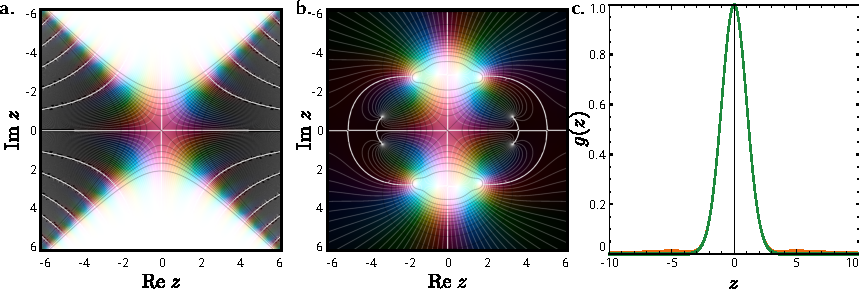
\includegraphics{figs/gr/GaussPade.pdf}
 \caption[Padé approximant for a Gaussian]{ \label{fig:GaussPade}
\textbf{Padé approximant for a Gaussian.}\small\\
\subA. Complex plot (\sec{f(z)}) of a Gaussian.
\subB. Its $(4,8)$ Padé approximant, showing 4 roots and 8 poles.
\subC. The two are compared as functions of a real variable for the Gaussian
(green), and its approximant (orange) showing additional side lobes.
}
\end{figure}
The Gaussian function is well behaved in the sense that it has no singularities
in the complex plane, however it diverges super-exponentially along the
imaginary axis which makes the complex contour method numerically unstable.
An alternative to using the Gaussian function would be to use one of its Padé
approximants.
A Padé approximant is the ratio of two power series of order $n$ and $m$
respectively.
This gives the function $n$ roots and $m$ simple poles in the complex plane.
The Gaussian is an even function, which means its approximant should have an
even number of roots.
It is also strictly positive, which is to say none of these roots lie on the
real axis, and indeed since real valued functions have their roots located at
complex conjugate pairs, the approximant needs to have a multiple of 4 roots to
preserve this property.
The number of poles is determined by similar argument, with the addition that
the function should go to zero for large values of $z$.
The asymptotic behaviour of the function is that of $z^{n-m}$, so by choosing
$(n=4, m=8)$, we return a strictly positive function that goes to zero with
$1/z^4$.
The $(4,8)$ Padé approximant is given as,
\begin{equation}
g_{4,8}(z) =
\frac{1 - \frac{z^2}{6} + \frac{z^4}{120} }
     {1 + \frac{z^2}{3} + \frac{z^4}{20} + \frac{z^6}{240} + \frac{z^8}{5760} }
\;,
\end{equation}
which is plotted alongside the Gaussian in \fig{GaussPade} in the complex
plane and on the real axis and can be seen to be a good match with the exception
of small side-lobes either side of the main peak.
Since this approximation has introduced $m=8$ simple poles into the complex
plane, explicit care must be taken that the contour integration of
\eq{neqKernel} does not pass over the singularities without taking into account
the residues as prescribed previously in the case of the Fermi function.

\begin{figure}
 \includegraphics{figs/gr/HotDist.pdf}
 \caption[Polarisability of a hot electron distribution]{\label{fig:HotDist}
\textbf{Polarisability of a hot electron distribution.}\small\\
\subA. A hot carrier distribution of a symmetrically excited Gaussian
distribution of electrons and holes over a quasiequilibrium background
simulating photoinversion
\subB. The optical conductivity of this is plotted, for occupations levels
$n_0$, (the height of the Gaussian) between $0$ and $0.5$. 
Both real (green) and imaginary (orange) parts of the conductivity change about
the pump frequency, $\ωpump$.
\subC. Plasmon dispersions and \subD. losses for this polarisability are also
plotted.
The curves noticeably kink about the pump frequency $\ωpump$.
}
\end{figure}
The polarisability $\Π[n]$, calculated from \eq{simpleHot} with a Padé
approximant, is explored with parameter values of
$\ħ\ωpump/2 = 2\μbar$,
$\γpump = 0.175 \μbar$,
$\Ttil = 0.05$, and
$\μe = \μh$
in \fig{HotDist} for peak carrier occupations between $0$ and $0.5$.
Firstly, in a), the dimensionless conductivity is plotted for external optical
excitation, i.e. $q \→ 0$, $\ω \in \reals$, where,
\begin{equation}
  \Zf \σs(\qtilAbs, \ωtil)
= i \αf \frac{g}{2} \frac{\ωtil}{\qtilAbs^2}
  \Πtil(\qtilAbs, \ωtil)
\;.
\end{equation}
It can be seen that the real part of the conductivity, which at zero pump is
flat for $\ω \gtrsim 1$ begins to dip for increased pump strength at
$\ω = \ωpump$.
The corresponding imaginary part is modified for all frequencies centred about
this point as the refractive index changes.
The conductivity drops to zero at $\ω = \ωpump$ as the sheet is pumped to
transparency at $n_0 = 0.5$.

\FigSub{HotDist}{.b} and .c plots the plasmon dispersion and loss for this
polarisability configuration for varying occupation number.
The plasmon dispersion shifts everywhere, but most markedly at
$\ω = \ωpump/2$ where the steepness dramatically increases.
Perhaps surprisingly, there is no reduction in the plasmon loss at any frequency
despite carrier pairs being available for recombination.
This can be attributed to the change in refractive index morphing the plasmon
dispersion to exclude it from regions where there is phase-space for stimulated
recombination.
% Is this gain (anti-)guiding, is this similar to what has been seen in SLL?
This can be seen in the gain region ($\ωtil < 1$), where the gain is due to
quasiequilibrium photoinversion.
Here the gain decreases, not because there is any more phase-space for
absorption processes, but rather that the plasmon dispersion curve has steepened
in this region, leaving less phase space for the quasiequilibrium recombination
processes.
As the pump increases, this also induces a sharp peak of the loss around
$\vF q = \ωpump/2$, again this is about where the plasmon dispersion has been
perturbed the most.

This section has shown that the polarisability can be calculated as a functional
of arbitrary carrier distributions as a function of a complex variable.
The resulting plasmon dispersions from quasiequilibrium and a hot carrier
model have been shown.
A change in the carrier distribution can have a dramatic impact on the plasmon
dispersion and loss, though provisionally from what has been seen, wherever
there is a spread in carriers, there is an increase in the phase space opened up
for absorption processes that is not matched with an increase in emission
processes.

\section{Spontaneous Emission Spectrum} \label{sec:sponEmit}
There are three fundamental single particle excitation processes occurring in graphene:
spontaneous emission, stimulated emission, and stimulated absorption.
Spontaneous emission occurs when an electron in a higher energy state
transitions to occupy an empty state of lower energy, and a plasmon is emitted
in the process.
In absorption, an incoming plasmon is converted into an electron-hole pair, or
equivalently raises a lower energy electron into a higher unoccupied level.
Whereas in stimulated emission an incoming plasmon forces an electron to
transition into an unoccupied lower energy state, releasing an additional
plasmon in the process that is coherent with the first.
It is the processes of absorption and stimulated emission that induce Landau
gain or loss in plasmons, and therefore are responsible for the imaginary part
of the plasmon frequency $\γpl$, which is the net decay rate (absorption minus
emission),
\begin{equation}
2\γpl = \γplabs - \γplemit
\;,
\end{equation}
where the factor of 2 is because $\γpl$ is a \emph{field} decay rate,
whereas $\γplabs$ and $\γplemit$ are \emph{intensity} decay rates.

Spontaneous emission on the other hand does not enter into $\γpl$ but can be
calculated indirectly from it by considering the rate of plasmon decay for each
wavevector labelled plasmon state.
\begin{equation}
\pd{\npl(q)}{\t} = -\γplemit(q) (\npl(q) + 1)
\;.
\end{equation}
This is a sum of a stimulated part ($\npl(q)$) and a spontaneous part ($+1$)
The spectral rate of emission within a frequency interval $[\ω, \ω + \d\ω]$ is
extracted by taking the partial sum over all wavevector states,
\begin{subequations}\subeq
\begin{align}
\Rspon &= \frac{1}{A}\sum_\q \γplemit(q) = \int_{0}^\infty \d\ω \: \Gpl(\ω) \\
&= \int_{0}^\infty \d\ω \: \pd{q(\ω)}{\ω} \frac{q(\ω)}{2\π} \γplemit
\big( q(\ω) \big)
\;,
\end{align}
\end{subequations}
with the plasmon density of states,
$\Dpl = \pd{q(\ω)}{\ω} {q(\ω)} / {2\π}$,
and the \emph{inverse} of the plasmon dispersion relation $q(\ω)$, such that
$q \big( \ωpl(q) \big) = q$.
The plasmon spectral recombination rate areal density, $\Gpl$ is therefore given
as the plasmon emission rate $\γplemit$ weighted to the density of states
$\Dpl$ for plasmons in the frequency interval $[\ω, \ω + \d\ω]$.
From here the particle (or hole) recombination rate may be extracted, by
dividing through by the particle areal density to give the recombination rate of
electrons:
\begin{equation}
\Γple = \Rspon / N(\μe, \T)
\;,
\end{equation}
where $N(\μe, \T)$ is the particle number density in the conduction band.

It is not necessarily obvious how to extract the emission and absorption rates,
$\γplemit$ and $\γplabs$.
For zero temperature, these rates are mutually exclusive, i.e.
$\γplabs = 0 \text{ for } \γplemit \neq 0$ and vice-versa, since in the regions
where there is phase space for absorption processes, there is none for emission.
This is to say, the rates can be expressed with step functions,
\begin{subequations}\subeq \label{eq:zeroTRates}
\begin{align}
\γplemit(q) &= -2 \γpl(q) \θ( \μbar   - \ħ\ω(q) ) \\
\γplabs (q) &=  2 \γpl(q) \θ( \ħ\ω(q) - \μbar   )
\;.
\end{align}
\end{subequations}
For finite temperatures and hot carrier distributions, where the regimes overlap
each other, the situation is complicated.
Looking at the Lindhard formula \eq{lindhard}, there is a sum of distribution
functions, which is equivalent to the sum of a Fermi function product for the
phase space of each process.
\begin{equation}
n(\έ^s_{\k}) - n(\έ^{s'}_{\k+\q}) =
\underbrace{
n(\έ^s_{\k}) \Big( 1 - n(\έ^{s'}_{\k+\q}) \Big)
}_\text{Absorption} -
\underbrace{
n(\έ^{s'}_{\k+\q}) \Big( 1 - n(\έ^s_{\k}) \Big)
}_\text{Stimulated Emission}
\;,
\end{equation}
which is to say, the polarisability itself can be split up into,
\begin{equation}
\Π[n](\q, \ω) = \Σabs[n](\q, \ω) - \Σemit[n](\q, \ω)
\;,
\end{equation}
with,
\begin{equation}
\Σemit[n](\q,\ωpl) = \frac{g}{A} \Im \sum_{s,s'=\pm} \sum_{\k}
M^{s s'}_{\k,\k+\q}
\frac{
n(\έ^{s'}_{\k+\q}) \Big( 1 - n(\έ^s_{\k}) \Big)
}
{\έ^s_{\k} - \έ^{s'}_{\k+\q} + \ħ\ωpl + \i\times0}
\;,
\end{equation}
and an equivalent term for $\Σabs$.

The rates for the two individual processes can be calculated approximatively by
a \emph{Fermi's golden rule} (\fgr) expression.
Borrowing from the low-loss approximation \eq{lowloss}, the expression,
\begin{equation}
\γpl \approx V_q \Im \Π(\ωpl, q) \bigg/ \Re
\left.\pd{\εRPA}{\ω}\right|_{\ω=\ωpl}
\;.
\end{equation}
$\Π(\ωpl, q)$ can be split into absorption and emission components\footnote{
This step is not exact either, as the polarisability $\Π$ enters into $\εRPA$,
though as we will see, it makes a good approximation.
}
using $2\γpl = \γplabs - \γplemit$,
\begin{subequations}\subeq
\begin{align}
\γplabs \approx 2 V_q \Σabs(\ωpl, q) \bigg/ \Re
\left.\pd{\εRPA}{\ω}\right|_{\ω=\ωpl}
\\ \label{eq:γplemit}
\γplemit \approx 2 V_q \Σemit(\ωpl, q) \bigg/ \Re
\left.\pd{\εRPA}{\ω}\right|_{\ω=\ωpl}
\;.
\end{align}
\end{subequations}
This approximation may fair better than the low-loss approximation, since we can
put in the exactly solved real part of the dispersion.
This expansion will still start to break down as the Fermi line is approached,
though the emission term will fare much better than the absorption since, at
least for quasiequilibrium at moderate temperatures, the emission rate
approaches zero before the dispersion hits the Fermi line.
From here the absorption term can be derived from the exact net term as
$\γplabs = 2\γpl + \γplemit$.

The emission partial polarisability can be put into integrable form,
assuming only interband recombination processes are significant, as,
\begin{equation}
\Σemit(q,\ω)=
\frac{g q^2}{8 \π \ħ} \frac{\θ(\ω-\vF q)}{\sqrt{\ω^2-\vF^2 q^2}}
\int\limits_{-1}^{+1} \d u \: \sqrt{1-u^2}
n \left( \frac{\ħ\ω + \ħ \vF q u}{2} \right)
\bar{n} \left( \frac{\ħ \ω - \ħ \vF q u}{2} \right)
\;.
\end{equation}
which is derived in the appendix of \cite{Page2015}.

\begin{figure}
 \includegraphics{figs/gr/SponZero.pdf}
 \caption[Spontaneous plasmon emission and electron recombination]{
 \label{fig:SponZero}
\textbf{Spontaneous plasmon emission and electron recombination.}\small\\
\subA. Plasmon spontaneous emission spectra, $\Gpltil$ and \subB. electron
recombination rates $\Γpletil$ at zero temperature.
Exact results derived from \cfpd curves (i) are plotted against approximate
results derived from \fgr for a classical Drude model (ii), \cfpd curves (iii),
and low-loss approximation.
Curves are dependent on carrier imbalance, $m$.
}
\end{figure}

The spontaneous emission is calculated and plotted in \fig{SponZero} for
zero temperature quasiequilibrium graphene, exactly (red lines) and in various
approximations.
Since for zero temperature, \eq{zeroTRates} holds and $\Gpl$ and $\Γple$ can be
calculated exactly [(i) in the figure] from the \cfpd using the directly
extracted $\γpl(q)$.
Three \fgr approximations are derived by calculating $\γplemit$ from
\eq{γplemit}, using the dispersion relations $\ωpl(q)$ from the classical Drude
model (ii), the \cfpd solution (iii), and the low-loss approximation;
curves which have been shown previously in \fig{PlasDisp}.
The exact result, obtained from the \cfpd will be used to test and
benchmark the appropriateness of \fgr solutions, which is important as
regimes where exact solutions cannot be obtained are explored.

The figure plots the dimensionless quantities
$\Gpltil = (\ħ\vF)^2\Gpl / \μbar^2$ and
$\Γpletil = \ħ\Γple / \μbar$,
which have the usual universality property\footnote{
$\Gpltil$ is scaled to the square of the energy scale $\μbar$ as it is an areal
density (\twod) quantity.
}.
Each set of curves in \figSub{SponZero}{.a} scans the spontaneous emission
spectrum over $\ωtil$ for varying levels of carrier inversion $m$.
The symmetrically inverted case $m=0$ acts as the envelope for each of the other
curves as the level of spontaneous emission drops with a reduction in inversion.
The curves all vanish to zero for $\ωtil > 1$ due to there being no phase space
outside this regime.
Of the approximative curves, the Drude model performs the worst, being a factor
of 5 slower than the exact solution.
This is due to a density of states that is an order of 10 times smaller than for
the other curves, despite having a raw emission rate $\γplemit$ that is larger
comparatively.
Using the low-loss approximation (iii) yields results that are the right order
of magnitude, but have spurious spikes in the curves which are a result of the
first order approximation overshooting when the dispersion curve passes near any
branch points.
The \cfpd dispersion approximation yields results that are most quantitatively
similar to the exact solution, though the match is not perfect and distinctive
dips are also observed near where the solution passes in the vicinity of branch
points.

In \figSub{SponZero}{.d}, each of the $\Gpltil$ curves are integrated over
frequency then scaled to the electron density to return the electron
recombination rate.
The equivalent procedure may be applied for holes and, due to particle-hole
symmetry, can be related as $\Γplhtil(m) = \Γpletil(-m)$.
The resulting curves are not themselves though symmetric about $m=0$ because for
electrons, for $m > 0$ they are the majority carrier, and for $m < 0$ the
minority and hence more sensitive to a change in carrier numbers.
The skew to the left indicates that the rate of electron recombination is
strongest when holes are the majority carrier, i.e. when for each electron, the
amount of holes available to recombine with is saturated.
The classical Drude limit has recombination rates a factor of 5 slower
than what is predicted using the exact formalism, and with
rates previously predicted in \cite{Rana2011}.
The other approximations work rather better in this picture, with any
inconsistencies that were present in the spectral form having been averaged out
in the recombination rate and largely matching the exact result.

In this formalism, carrier recombination rates are predicted to be a factor 5
faster than previously calculated.
When using representative energy scales, e.g. $\μbar = 0.2\eV$ yield
recombination times of $34\fs$ (at $m=0$).

Nonequilibrium Plasmon emission must therefore be considered as an important
channel for interband carrier recombination alongside the optical phonon
emission
\cite{Butscher2007,Rana2009,Wang2010,Yan2013}
and Auger recombination channels
\cite{Rana2007,Winzer2012,Tomadin2013,Brida2013}
when the dynamics of hot carriers in graphene are analysed
\cite{Breusing2011,Li2012,Gierz2013}.

\subsection{Recombination Rates at Finite Temperature and Collision Loss}
Armed with a reliable way to estimate spontaneous emission and \mdf
recombination rates, it remains to investigate how this changes with the
inclusion of finite temperature, or collision losses.

\begin{figure}
 \includegraphics{figs/gr/SponTemp.pdf}
 \caption[Impact of temperature and collisions on spontaneous emission]
 {\label{fig:SponTemp}
 \textbf{Impact of temperature and collisions on spontaneous emission.}\small\\
Plasmon gain spectrum $\Gpltil(\ωtil)$ for intrinsic graphene ($m=0$) for:
\subA.
collision losses spanning $\τtil^{-1} \in [0,0.08]$, and \subB. temperatures
spanning $\Ttil^{-1} \in [0,0.1]$. Electron recombination rates over the same
temperature range are plotted in \subC over carrier imbalance $m$.
}
\end{figure}

By including collision loss and finite temperature effects, \eq{zeroTRates} no
longer holds, as the loss rate $\γpl$ is now not entirely due to recombination,
with added contributions from collision and Landau damping loss bleeding in.
In this situation the \fgr approximation of \eq{γplemit} must be used.
Curves for $m=0$ (representing the envelope) are plotted in the \cfpd \fgr
approximation for finite collision rates in \figSub{SponTemp}{.a} and finite
temperature in \figSub{SponTemp}{.b}.
In the case of collision loss, the rates hardly change at all.
This is because collision loss, although increasing the plasmon loss, is not a
recombination mechanism, and therefore does not contribute in the \fgr
expansion.
Any changes, including the smoothing out of the kink in the curve, are due to
the small changes in the dispersion curve from which the \fgr is calculated.

The situation for a finite temperature is quite different.
The character of the the emission rate $\γplemit$ shows a blueshift as the hard
edge at $\ωtil = 1$ for $\T = 0$ softens out to finite values for $\ωtil > 1$
as the phase space opens, much as was the case for the stimulated emission rates
(\fig{LowTemp}).
While the peak value of spontaneous emission decreases with temperature, the
spectrum as a whole broadens.
This can be seen most clearly in the \mdf recombination rates, which increase
with temperature for all values of $m$.
Again, when electrons are the minority carrier, their recombination rates are
more sensitive to changes in temperature, with increased phase space for
increased temperature.

The recombination time drops as temperature increases, from a value of $34\fs$
at zero temperature, as reported in the previous section, to a peak value of
$1/\Γple = 18\fs$ for $\T = 230\K$ and $m=-0.5$.

Summarising the results of this section, \fgr approximations of the emission and
absorption components of the plasmon rates have been shown.
The accuracy of these is critical on using the real part of the exactly solved
\cfpd solution, with approximative solutions (classical Drude model, and \rpa
polarisability in a low-loss approximation) giving results that are either
factors out, or with spurious features.
The emission rate can be used to calculate the spontaneous emission rates and
derived carrier recombination rates, which are found to be sensitive to
temperature, but insensitive to levels of collision losses.
The recombination rates are significantly faster than previously predicted and
must be considered in an analysis of carrier relaxation.

\section{Carrier Relaxation Dynamics} \label{sec:npe}
It was established in the previous section that spontaneous plasmon emission is
an ultrafast process in photoinverted graphene, with rates exceeding that of
optical phonon emission by orders of magnitude \cite{Rana2011}.
The resulting rates for carrier recombination indicate that plasmon emission may
be the dominant decay channel for nonequilibrium carrier relaxation in
graphene, a process that had been previously been attributed to Auger
recombination (\ar) \cite{Breusing2011,Brida2013}, which is subject to debate as
\ar processes are suppressed under \rpa dynamic screening models
\cite{Tomadin2013,Tielrooij2013}.

The recombination rates presented in the previous section are the instantaneous
values based on a fixed carrier distribution, whereas carrier recombination will
precisely seek to change the distribution over time.
In order to accurately predict how \emph{nonequilibrium plasmon emission}
(\npe) affects the carrier dynamics, a time-domain study of the carrier and
plasmon system becomes necessary together with additional recombination
pathways such as optical phonon emission, which may interplay and seek to take
heat out of the system.

For this section, the carrier system is assumed to relax instantaneously to
quasiequilibrium characterised by chemical potentials $\μe$ and $\μh$, for
electrons and holes respectively in the conduction and valence bands, and a
common carrier temperature $\Tc$, which feeds into Fermi carrier distributions
in each band as described in \sec{quasieq}.
Meanwhile the bosonic excitations, plasmons and optical phonons, are resolved by
wavevector $\nβ(\q)$ for each species bath, $\β$.

The carrier system's number and energy density moments, $\Ne$, $\Nh$, and $U$
evolve in time as driven by an external optical excitation pump term and due to
relaxation terms that couple to the boson baths.
\begin{subequations}\subeq
\begin{align}
\Ndote = \Ndoth &= \NdotPump - \NdotRel \\
\Udot &= \UdotPump - \UdotRel
\;.
\end{align}
\end{subequations}
Carriers are always generated pairwise as an electron and a hole, which results
in their rates being equal.

Assuming the system is pumped by a normally incident quasi-monochromatic,
$\ħ\ωpump$, planewave with a slowly varying envelope $I(\t)$, then the carrier
pairs excited and energy dissipated into the system is given by,
\begin{subequations}\subeq
\begin{align}
\NdotPump &= \Re [ \σsinter(\ω) ] |E(t)|^2 / (2\ħ\ω) \\
\UdotPump &= \Re [ \σs(\ω) ] |E(t)|^2 / 2 ,
\end{align}
\end{subequations}
where $\σs(\ω)$ is the optical conductivity ($q = 0$) as in \eq{condpol},
$\σsinter$ is the contribution to the sheet conductivity from interband
processes only, and $E(t)$ is the in plane component of the electric field
generated from a beam with an input intensity of $I(t)$, given as,
\begin{equation}
|E(t)|^2 =  2 \Zf \left|
\frac{1}{1 + \Zf \σs(\ω) / 2}
\right|^2
I(t)
\;,
\end{equation}
as derived from the \tmm formalism in \sec{stratmed}.

The system relaxes according to Boltzmann collision integrals, which account for
intraband scattering and interband recombination and pair generation processes.
Each boson field reservoir, $\β$, contributes to the number and energy density
relaxation rates.
Whereas only interband processes affect the number density, as these are the
processes that produce electron-hole pairs, both inter- and intraband processes
($\λ \in \{\ee,\hh,\eh\}$) relax the energy density,
\begin{subequations}\subeq
\begin{align}
\NdotRel &= \sum_\β \Rβ \\
\UdotRel &= \sum_{\β,\λ} \Sβλ
\;.
\end{align}
\end{subequations}
These rates themselves are summed over wavevector resolved processes, over each
band combination,
\begin{subequations}\subeq
\begin{align}
\Rβ &= \frac{1}{A} \sum_\q \rβeh(\q)\\
\Sβλ &= \frac{1}{A} \sum_\q \ħ\ω_\β(\q) \rβλ(\q)
\;.
\end{align}
\end{subequations}
with $\rβλ(\q)$ being the net spectral emission rate, including both
stimulated and spontaneous processes,
\begin{equation} \label{eq:netSER}
\rβλ(\q) = \γemit(\q) [\nβ(\q) + 1] - \γabs(\q) \nβ(\q)
\;.
\end{equation}
The bosonic fields themselves then relax via this interaction with the carrier
system, but additionally through decay processes through other channels
characterised by a relaxation rate $\nβdotrel(\q)$,
\begin{equation}
\nβdot = \sum_\λ \rβλ(\q) - \nβdotrel(\q)
\;.
\end{equation}
These additional relaxation processes can be phenomenologically modelled by a
characteristic time $\τβ$,
\begin{equation}
\nβdotrel(\q) = \τβ^{-1} \left[\nβ(\q) - \nβeq(\q,\Tamb)\right]
\;,
\end{equation}
where $\nβeq(\q,\Tamb)$ is the equilibrium distribution at an ambient
temperature $\Tamb$.

Initially a study of the carrier/plasmon system in isolation will be presented,
then optical phonons will be included.
The initial conditions for each simulation are the same; a pulse of fluence
$133 \μJ / \cm^2$ with frequency $\ħ\ω = 1\eV$ is incident on ambient
temperature intrinsic equilibrium graphene.
During excitation, in order that each initialisation is the same, relaxation
processes are turned off.
This leaves the system in an inverted state with $\μe = \μh \approx 0.3\eV$ and
$\Tc \approx 0.2\eV/\kB \: (2320\K)$.
As the system starts intrinsically doped $\μe = \μh$ and all carrier excitations
are pairwise, the electron and hole chemical potentials will remain equal, i.e.
a carrier imbalance of $m=0$, throughout the simulation.
The plasmon system is resolved isotropically in wavevector, i.e.
$\npl(\q) = \npl(q)$.

\begin{figure}
 \includegraphics{figs/gr/NPERelax.pdf}
 \caption[Relaxation dynamics of coupled plasmon and carrier system]{
 \label{fig:NPERelax}
 \textbf{Relaxation dynamics of coupled plasmon and carrier system.}\small\\
\subA. Chemical potential (Green) and temperature (orange) of the carrier system
relaxing over time.
Solid lines are for a collision time $\τpl = 100\fs$ while shaded areas vary
from this in the range $\τpl \in [10,500]\fs$.
\\
\subB. shows the wavevector resolved plasmon occupation $\npl(q)$.
Black dashed lines mark the transition from absorption to emission.
}
\end{figure}

\subsection{Relaxation Via the Plasmon Channel}
The relaxation after excitation of the isolated carrier/plasmon system
(without optical phonons) is considered for a range of collision rates $\τpl$ in
the range $[10, 500]\fs$.
\Fig{NPERelax} shows how, in the first $1\ps$ after excitation, the carrier
system (a) and plasmon system (b) relaxes.
There is a sharp drop in inversion in the first $50\fs$ as the initially empty
plasmon bath is populated via interband recombination of carrier pairs.
The temperature correspondingly rises in this interval, which although the
energy density is dropping due to conversion to plasmons, the temperature must
rise such that the highest occupied carriers still have a probability of
occupation.
Plasmons may only be emitted at energies below $2\μ$, i.e. for $\γpl(\q) = 0$,
above this they are reabsorbed; the Fermi-edge drops over time meaning that
plasmons that were previously emitted may now be reabsorbed.
This reabsorption also increases the temperature, as there are many
electron-hole pair combinations that each plasmon may decay into, conserving
energy and momentum, despite having been created from a single particular
pair; this will seek to smear out the carrier distribution.
Over the next $200\fs$ the recombination rates slow down as inversion is
converted into temperature reducing the net emission of plasmons as in
\fig{TempScan}.
The dropping Fermi-edge means that plasmons that had been emitted
are being reabsorbed into the carrier system.
This slows down the decay rate of both the energy and number density which may
be described as a \emph{plasmon emission bottleneck}.
With an increasing collision loss, more plasmons are removed from the system, 
meaning that their energy is not being converted into electron-hole pairs,
lifting the bottleneck and allowing the carrier inversion to decay more
quickly.
This is most obviously noticed by comparing the steepness of the
outermost curves for the carrier temperature and chemical potential with
inversion lingering at $\μ = 0.1\eV$ for $\τpl = 500\fs$ but quickly depleting
at $\τpl = 10\fs$.

\subsection{Optical Phonons} \label{sec:optPhonons}
\begin{figure}
 \includegraphics{figs/gr/NPERelaxPhon.pdf}
 \caption[Relaxation dynamics of carriers coupled plasmons and phonons]{
 \label{fig:NPERelaxPhon}
 \textbf{Relaxation dynamics of carriers coupled plasmons and phonons.}\small\\
\subA. Carrier temperature and chemical potential of carriers coupled only to
phonons, also shows the relaxation of phonon temperatures over time.
\subB. re-introduces plasmons, along with phonons, for varying collision times
$\τpl$.
\subC. and \subD. show extracted parameters ($A_i$, $\τ_i$) of a tri-exponential
fit of $\μ(t)$ for plasmons in isolation, and plasmons and phonons.
}
\end{figure}

Phonons also play a role in the relaxation of a hot carrier distribution
\cite{Wang2010},
being a channel for both intraband scattering \cite{Breusing2011} and interband
pair generation / recombination \cite{Rana2009}.
\emph{Longitudinal optical} (\LO) and \emph{transverse optical} (\TO) phonons
are the dominant channels for coupling to the carrier system.
They couple about the Γ and K symmetry points, allowing intra- and inter-valley
transitions respectively; about these points they are quasi-dispersion free
having a single frequency.
These are the \ΓO and \KO phonons, for which $\έΓO = 196\meV$,
$\έKO = 160\meV$.
There is also an acoustic phonon that couples at the K point
in this manner, \KA with $\έKA = 120\meV$.
Closed form expressions for the net spectral emission rates, as in \eq{netSER},
can be derived due to the dispersion free nature of the modes, and are presented
in the supplementary material of Ref~\cite{Hamm2015}.

\FigSub{NPERelaxPhon}{.a} shows how the carrier system relaxes in the
presence of only the phonons, i.e. with plasmons not included.
The phonons are modelled to follow a Bose-Einstein distribution with a separate
temperature for each phonon species.
Since each species is mono-energetic, the temperature will uniquely determine
the occupation number of that species.
Such description assumes an instantaneous relaxation of the phonons to be
uniformly distributed over wavevector.
The phonon relaxation time is assumed to be $\τph = 2.5\ps$ \cite{Wang2010}.

In the first $500\fs$ the carrier temperature drops accompanied by an increase
in chemical potential and a rise in phonon temperatures.
This is indicative of intraband scattering, where the number density stays the
same, but energy is transferred from the carriers to phonons.
Once the phonon and carrier temperatures match, they then largely follow each
other, slowly decreasing as phonons are emitted from interband recombination of
carriers.

Next plasmons and phonons are simulated together, the trace of carrier and
phonon configuration is given in \figSub{NPERelaxPhon}{.b}.
Initially inversion drops sharply as plasmons are emitted, but this is not
accompanied by a sharp rise in carrier temperature, as was the case with
plasmons alone, as the coupling with phonons removes excess temperature from the
carrier plasma through intraband emission.
Again, once the carrier and phonon temperatures have equalised after around
$1\ps$, the inversion slowly drains, albeit, in contrast to with phonons alone,
the chemical potential has by now been significantly cut.
With an increase in the plasmon decay rate, energy is removed from the system
faster, though with the phonons now acting as an efficient channel to extract
heat, this effect is less sensitive to the decay rate than with plasmons alone.

Further inferences can be made by examining the characteristic of the chemical
potential drop in more detail.
A tri-exponential function,
$\μ = \μ_0 \sum_{i=1}^3 A_i \exp(-t / \τ_i)$,
can be fit to the time evolution.
\FigSub{NPERelaxPhon}{.c} shows this fit for both \npe alone and \npe with
phonons, as plasmon collision loss varies.
The timescales that emerge ($\τ_1$, $\τ_2$, $\τ_3$) separate out into distinct
values that are largely independent on the collision loss.
The fastest timescale, $\τ_1 \approx 0.03\ps$ represents the filling of the
initially empty plasmon bath via spontaneous recombination of electron-hole
pairs.
The amplitude, $A_1$, of this timescale is steady for $\τpl > \τ_1$, though in
the opposite limit, where plasmons are absorbed at a faster rate than they are
created, the amplitude shoots up as most of the energy is extracted from the
system in this way.
The second timescale $\τ_2 \approx 0.3\ps$ is associated with the conversion of
inversion to temperature, by emitting plasmons below the Fermi-edge, the edge
dropping, and the same plasmons re-absorbing above it.
The amplitude $A_2$, of this process drops as $A_1$ rises when plasmons are
quickly dissipated for $\τpl < \τ_1$, this is because there will be no plasmons
in the bath to re-absorb back into the carrier system.
The final rate $\τ_3$ represents the remaining drain of energy as the saturated
plasma bath depletes.
As the collision loss increases, $\τpl \gtrsim 0.2\ps $, the proportion of the
inversion lost through this mechanism increases, thereby depleting the next
slowest rate amplitude $A_2$.
This channel is the only one whose rate is significantly affected by the
inclusion of phonons, with the characteristic time $\τ_3$ universally
increasing; this can be attributed to the phonons being a separate store of
energy that is passed through before exiting the system.

Overall, the dependence on collision loss only affects the dynamics
significantly if it is small enough to empty the plasmon bath faster than it is
filled, at $\τpl \lesssim 0.2\ps$.
The addition of phonons into the model however most strongly influences the
dynamics by slowing down the decay of inversion and reducing its dependence on
the plasmon relaxation rate.

This establishes that \npe acts as an efficient mechanism for the equilibration
of thermal photoinverted graphene.
Hot electron-hole pairs may recombine creating a plasmon, removing energy and
carriers from the \mdf plasma.
This energy is re-distributed back to the carrier system and through phonon
channels to eventually be removed from the system as the plasmon bath is
depleted due to electron collisions.
The predictions are self-consistent and in agreement with experimental findings
\cite{Li2012} without requiring arbitrary tuning.

\section{Conclusions}
This chapter has introduced a method of calculating the polarisability of
graphene for arbitrary carrier distributions in the Dirac cone approximation.
This has allowed for the calculation of the complex frequency plasmon dispersion
curves, which are exact solutions of the poles of the Coulomb potential in \rpa.
The complex nature of the solution encodes in its imaginary part the rates of
loss and gain for plasmons in regions where there is coupling through
absorption and stimulated emission to the \mdf plasma.
By calculating the emission spectrum, this work gives
indication that plasmons with gain can indeed exist in graphene under realistic
conditions.

The resilience of the plasmons under conditions of collision loss, finite
temperature, and chemical doping has been demonstrated.
The modal loss added by the inclusion of collisions is proportional to the
inverse of the collisional lifetime, whereas the effects of temperature and
doping is to blueshift the frequency of the peak loss rate.
The dispersion of the plasmons is largely unaffected by collisions and low
temperatures, but sensitive to doping, exhibiting a critical splitting in the
families of curves observed.
The plasmons of hot nonequilibrium carriers are shown to have strong dependency
on the carrier distribution.

Spontaneous emission, that accompanies the stimulated gain, is also described in
this model.
A Fermi's golden rule scheme allows for the extraction of the spontaneous
plasmon emission spectrum, but also for the carrier recombination rates.
These are calculated under the effects of collision, temperature, and
doping.
While collisions do not contribute to this channel, temperature and doping have
a strong influence.
The rates calculated for nonequilibrium graphene are shown to be a factor 5
times faster than previously estimated.
This suggests that plasmons play a key role in the dynamics of hot carrier
inversion decay, that has been observed in pump-probe and \trarpes experiments.

The dynamics of carrier relaxation is investigated in interaction with plasmon
and phonon reservoirs.
It is shown that by emitting into the plasmon channels, energy can be removed
from the carrier system on $100\fs$ timescales, which is consistent with recent
experimental results \cite{Breusing2011,Li2012}.
